\documentclass[twoside]{book}

% Packages required by doxygen
\usepackage{calc}
\usepackage{doxygen}
\usepackage{graphicx}
\usepackage[utf8]{inputenc}
\usepackage{makeidx}
\usepackage{multicol}
\usepackage{multirow}
\usepackage{textcomp}
\usepackage[table]{xcolor}

% Font selection
\usepackage[T1]{fontenc}
\usepackage{mathptmx}
\usepackage[scaled=.90]{helvet}
\usepackage{courier}
\usepackage{amssymb}
\usepackage{sectsty}
\renewcommand{\familydefault}{\sfdefault}
\allsectionsfont{%
  \fontseries{bc}\selectfont%
  \color{darkgray}%
}
\renewcommand{\DoxyLabelFont}{%
  \fontseries{bc}\selectfont%
  \color{darkgray}%
}

% Page & text layout
\usepackage{geometry}
\geometry{%
  a4paper,%
  top=2.5cm,%
  bottom=2.5cm,%
  left=2.5cm,%
  right=2.5cm%
}
\tolerance=750
\hfuzz=15pt
\hbadness=750
\setlength{\emergencystretch}{15pt}
\setlength{\parindent}{0cm}
\setlength{\parskip}{0.2cm}
\makeatletter
\renewcommand{\paragraph}{%
  \@startsection{paragraph}{4}{0ex}{-1.0ex}{1.0ex}{%
    \normalfont\normalsize\bfseries\SS@parafont%
  }%
}
\renewcommand{\subparagraph}{%
  \@startsection{subparagraph}{5}{0ex}{-1.0ex}{1.0ex}{%
    \normalfont\normalsize\bfseries\SS@subparafont%
  }%
}
\makeatother

% Headers & footers
\usepackage{fancyhdr}
\pagestyle{fancyplain}
\fancyhead[LE]{\fancyplain{}{\bfseries\thepage}}
\fancyhead[CE]{\fancyplain{}{}}
\fancyhead[RE]{\fancyplain{}{\bfseries\leftmark}}
\fancyhead[LO]{\fancyplain{}{\bfseries\rightmark}}
\fancyhead[CO]{\fancyplain{}{}}
\fancyhead[RO]{\fancyplain{}{\bfseries\thepage}}
\fancyfoot[LE]{\fancyplain{}{}}
\fancyfoot[CE]{\fancyplain{}{}}
\fancyfoot[RE]{\fancyplain{}{\bfseries\scriptsize Generated on Sat Aug 10 2013 09:13:18 for Programming project 3 by Doxygen }}
\fancyfoot[LO]{\fancyplain{}{\bfseries\scriptsize Generated on Sat Aug 10 2013 09:13:18 for Programming project 3 by Doxygen }}
\fancyfoot[CO]{\fancyplain{}{}}
\fancyfoot[RO]{\fancyplain{}{}}
\renewcommand{\footrulewidth}{0.4pt}
\renewcommand{\chaptermark}[1]{%
  \markboth{#1}{}%
}
\renewcommand{\sectionmark}[1]{%
  \markright{\thesection\ #1}%
}

% Indices & bibliography
\usepackage{natbib}
\usepackage[titles]{tocloft}
\setcounter{tocdepth}{3}
\setcounter{secnumdepth}{5}
\makeindex

% Hyperlinks (required, but should be loaded last)
\usepackage{ifpdf}
\ifpdf
  \usepackage[pdftex,pagebackref=true]{hyperref}
\else
  \usepackage[ps2pdf,pagebackref=true]{hyperref}
\fi
\hypersetup{%
  colorlinks=true,%
  linkcolor=blue,%
  citecolor=blue,%
  unicode%
}

% Custom commands
\newcommand{\clearemptydoublepage}{%
  \newpage{\pagestyle{empty}\cleardoublepage}%
}


%===== C O N T E N T S =====

\begin{document}

% Titlepage & ToC
\hypersetup{pageanchor=false}
\pagenumbering{roman}
\begin{titlepage}
\vspace*{7cm}
\begin{center}%
{\Large Programming project 3 }\\
\vspace*{1cm}
{\large Generated by Doxygen 1.8.4}\\
\vspace*{0.5cm}
{\small Sat Aug 10 2013 09:13:18}\\
\end{center}
\end{titlepage}
\clearemptydoublepage
\tableofcontents
\clearemptydoublepage
\pagenumbering{arabic}
\hypersetup{pageanchor=true}

%--- Begin generated contents ---
\chapter{Hierarchical Index}
\section{Class Hierarchy}
This inheritance list is sorted roughly, but not completely, alphabetically\-:\begin{DoxyCompactList}
\item \contentsline{section}{Best\-Canvas}{\pageref{class_best_canvas}}{}
\item \contentsline{section}{Canny}{\pageref{class_canny}}{}
\item \contentsline{section}{Canvas}{\pageref{class_canvas}}{}
\begin{DoxyCompactList}
\item \contentsline{section}{Bezier\-Path\-Canvas}{\pageref{class_bezier_path_canvas}}{}
\item \contentsline{section}{Decal\-Canvas}{\pageref{class_decal_canvas}}{}
\item \contentsline{section}{Shroud\-Canvas}{\pageref{class_shroud_canvas}}{}
\item \contentsline{section}{Triangle}{\pageref{class_triangle}}{}
\end{DoxyCompactList}
\item \contentsline{section}{Color\-Converter}{\pageref{class_color_converter}}{}
\item \contentsline{section}{Config\-Reader}{\pageref{class_config_reader}}{}
\item \contentsline{section}{Coord}{\pageref{struct_coord}}{}
\item \contentsline{section}{Decal}{\pageref{class_decal}}{}
\item Fitness\begin{DoxyCompactList}
\item \contentsline{section}{Image\-Fitness}{\pageref{class_image_fitness}}{}
\end{DoxyCompactList}
\item Function\begin{DoxyCompactList}
\item \contentsline{section}{Draw2}{\pageref{class_draw2}}{}
\item \contentsline{section}{Draw4}{\pageref{class_draw4}}{}
\item \contentsline{section}{Draw6}{\pageref{class_draw6}}{}
\item \contentsline{section}{Draw\-Color\-Triangle}{\pageref{class_draw_color_triangle}}{}
\item \contentsline{section}{Draw\-Gray\-Triangle}{\pageref{class_draw_gray_triangle}}{}
\item \contentsline{section}{Prog2}{\pageref{class_prog2}}{}
\item \contentsline{section}{Prog3}{\pageref{class_prog3}}{}
\item \contentsline{section}{Prog4}{\pageref{class_prog4}}{}
\end{DoxyCompactList}
\item \contentsline{section}{H\-S\-V}{\pageref{struct_h_s_v}}{}
\item \contentsline{section}{Mask\-Maker}{\pageref{class_mask_maker}}{}
\item \contentsline{section}{Palette}{\pageref{class_palette}}{}
\item \contentsline{section}{Pixel}{\pageref{class_pixel}}{}
\item \contentsline{section}{Ralph}{\pageref{class_ralph}}{}
\item Return\-Data\begin{DoxyCompactList}
\item \contentsline{section}{Return\-Float}{\pageref{class_return_float}}{}
\item \contentsline{section}{Return\-Func}{\pageref{class_return_func}}{}
\item \contentsline{section}{Return\-Root}{\pageref{class_return_root}}{}
\end{DoxyCompactList}
\item \contentsline{section}{R\-G\-B}{\pageref{struct_r_g_b}}{}
\item \contentsline{section}{Target}{\pageref{class_target}}{}
\item Terminal\begin{DoxyCompactList}
\item \contentsline{section}{Rand\-Float}{\pageref{class_rand_float}}{}
\end{DoxyCompactList}
\end{DoxyCompactList}

\chapter{Class Index}
\section{Class List}
Here are the classes, structs, unions and interfaces with brief descriptions\-:\begin{DoxyCompactList}
\item\contentsline{section}{\hyperlink{class_best_canvas}{Best\-Canvas} }{\pageref{class_best_canvas}}{}
\item\contentsline{section}{\hyperlink{class_bezier_path_canvas}{Bezier\-Path\-Canvas} }{\pageref{class_bezier_path_canvas}}{}
\item\contentsline{section}{\hyperlink{class_canny}{Canny} }{\pageref{class_canny}}{}
\item\contentsline{section}{\hyperlink{class_canvas}{Canvas} }{\pageref{class_canvas}}{}
\item\contentsline{section}{\hyperlink{class_color_converter}{Color\-Converter} }{\pageref{class_color_converter}}{}
\item\contentsline{section}{\hyperlink{class_config_reader}{Config\-Reader} }{\pageref{class_config_reader}}{}
\item\contentsline{section}{\hyperlink{struct_coord}{Coord} }{\pageref{struct_coord}}{}
\item\contentsline{section}{\hyperlink{class_decal}{Decal} }{\pageref{class_decal}}{}
\item\contentsline{section}{\hyperlink{class_decal_canvas}{Decal\-Canvas} }{\pageref{class_decal_canvas}}{}
\item\contentsline{section}{\hyperlink{class_draw2}{Draw2} }{\pageref{class_draw2}}{}
\item\contentsline{section}{\hyperlink{class_draw4}{Draw4} }{\pageref{class_draw4}}{}
\item\contentsline{section}{\hyperlink{class_draw6}{Draw6} }{\pageref{class_draw6}}{}
\item\contentsline{section}{\hyperlink{class_draw_color_triangle}{Draw\-Color\-Triangle} }{\pageref{class_draw_color_triangle}}{}
\item\contentsline{section}{\hyperlink{class_draw_gray_triangle}{Draw\-Gray\-Triangle} }{\pageref{class_draw_gray_triangle}}{}
\item\contentsline{section}{\hyperlink{struct_h_s_v}{H\-S\-V} }{\pageref{struct_h_s_v}}{}
\item\contentsline{section}{\hyperlink{class_image_fitness}{Image\-Fitness} }{\pageref{class_image_fitness}}{}
\item\contentsline{section}{\hyperlink{class_mask_maker}{Mask\-Maker} }{\pageref{class_mask_maker}}{}
\item\contentsline{section}{\hyperlink{class_palette}{Palette} }{\pageref{class_palette}}{}
\item\contentsline{section}{\hyperlink{class_pixel}{Pixel} }{\pageref{class_pixel}}{}
\item\contentsline{section}{\hyperlink{class_prog2}{Prog2} }{\pageref{class_prog2}}{}
\item\contentsline{section}{\hyperlink{class_prog3}{Prog3} }{\pageref{class_prog3}}{}
\item\contentsline{section}{\hyperlink{class_prog4}{Prog4} }{\pageref{class_prog4}}{}
\item\contentsline{section}{\hyperlink{class_ralph}{Ralph} }{\pageref{class_ralph}}{}
\item\contentsline{section}{\hyperlink{class_rand_float}{Rand\-Float} }{\pageref{class_rand_float}}{}
\item\contentsline{section}{\hyperlink{class_return_float}{Return\-Float} }{\pageref{class_return_float}}{}
\item\contentsline{section}{\hyperlink{class_return_func}{Return\-Func} }{\pageref{class_return_func}}{}
\item\contentsline{section}{\hyperlink{class_return_root}{Return\-Root} }{\pageref{class_return_root}}{}
\item\contentsline{section}{\hyperlink{struct_r_g_b}{R\-G\-B} }{\pageref{struct_r_g_b}}{}
\item\contentsline{section}{\hyperlink{class_shroud_canvas}{Shroud\-Canvas} }{\pageref{class_shroud_canvas}}{}
\item\contentsline{section}{\hyperlink{class_target}{Target} }{\pageref{class_target}}{}
\item\contentsline{section}{\hyperlink{class_triangle}{Triangle} }{\pageref{class_triangle}}{}
\end{DoxyCompactList}

\chapter{Class Documentation}
\hypertarget{class_best_canvas}{\section{Best\-Canvas Class Reference}
\label{class_best_canvas}\index{Best\-Canvas@{Best\-Canvas}}
}
\subsection*{Public Member Functions}
\begin{DoxyCompactItemize}
\item 
\hypertarget{class_best_canvas_ad182d4690d4551842643aebecc7c4855}{{\bfseries Best\-Canvas} (\hyperlink{class_target}{Target} $\ast$target, color\-\_\-t bg)}\label{class_best_canvas_ad182d4690d4551842643aebecc7c4855}

\item 
\hypertarget{class_best_canvas_a8fe1a93900c9c241d180cc4302724458}{{\bfseries Best\-Canvas} (\hyperlink{class_target}{Target} $\ast$target, color\-\_\-t bg\-\_\-\-Red, color\-\_\-t bg\-\_\-\-Green, color\-\_\-t bg\-\_\-\-Blue)}\label{class_best_canvas_a8fe1a93900c9c241d180cc4302724458}

\item 
\hypertarget{class_best_canvas_a132c5ae0ba4a64d861e0f02f4318f4cb}{void {\bfseries set\-R\-G\-B\-Pixel} (int offset, \hyperlink{struct_r_g_b}{R\-G\-B} pixel)}\label{class_best_canvas_a132c5ae0ba4a64d861e0f02f4318f4cb}

\item 
\hypertarget{class_best_canvas_a596f525da74cfb4f889ceca87a9cf4f6}{void {\bfseries set\-H\-S\-V\-Pixel} (int offset, \hyperlink{struct_h_s_v}{H\-S\-V} pixel)}\label{class_best_canvas_a596f525da74cfb4f889ceca87a9cf4f6}

\item 
\hypertarget{class_best_canvas_abd9c06a1c0304bec04a5060f31f6d9b8}{\hyperlink{struct_r_g_b}{R\-G\-B} {\bfseries get\-R\-G\-B\-Pixel} (\hyperlink{struct_coord}{Coord} c)}\label{class_best_canvas_abd9c06a1c0304bec04a5060f31f6d9b8}

\item 
\hypertarget{class_best_canvas_ae973df7ff7f90693cca4b883ccde1d59}{\hyperlink{struct_h_s_v}{H\-S\-V} {\bfseries get\-H\-S\-V\-Pixel} (\hyperlink{struct_coord}{Coord} c)}\label{class_best_canvas_ae973df7ff7f90693cca4b883ccde1d59}

\end{DoxyCompactItemize}


The documentation for this class was generated from the following files\-:\begin{DoxyCompactItemize}
\item 
Best\-Canvas.\-h\item 
Best\-Canvas.\-cpp\end{DoxyCompactItemize}

\hypertarget{class_bezier_path_canvas}{\section{Bezier\-Path\-Canvas Class Reference}
\label{class_bezier_path_canvas}\index{Bezier\-Path\-Canvas@{Bezier\-Path\-Canvas}}
}
Inheritance diagram for Bezier\-Path\-Canvas\-:\begin{figure}[H]
\begin{center}
\leavevmode
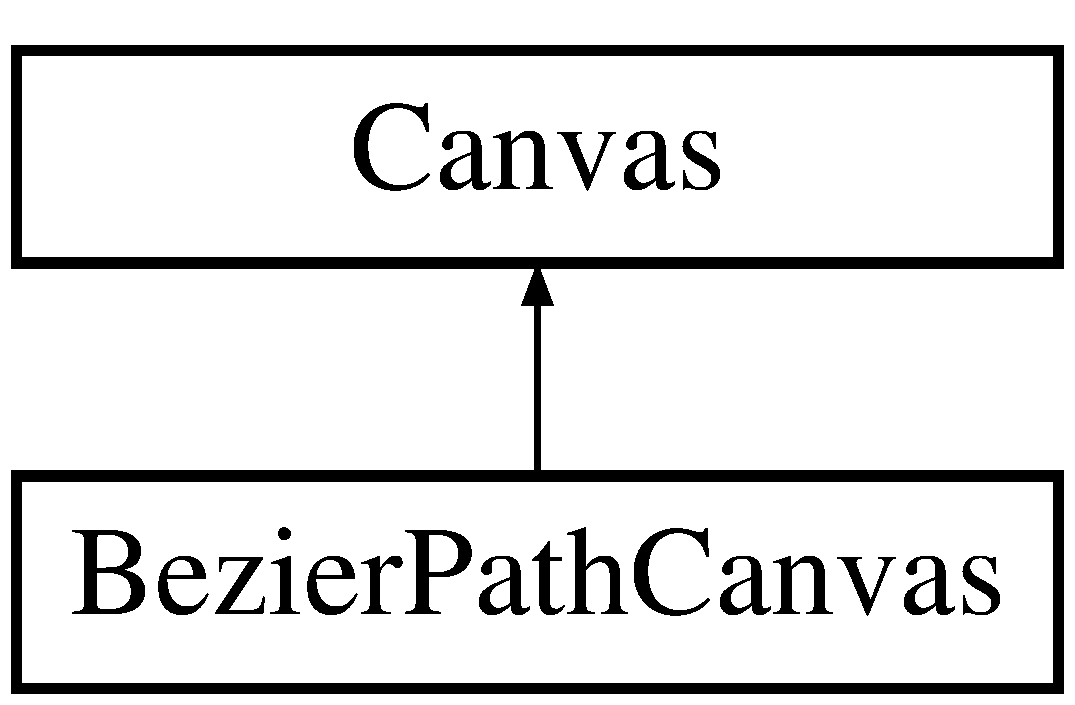
\includegraphics[height=2.000000cm]{class_bezier_path_canvas}
\end{center}
\end{figure}
\subsection*{Public Member Functions}
\begin{DoxyCompactItemize}
\item 
\hypertarget{class_bezier_path_canvas_ae24f243f5019dbd8fcab3312ffbf1188}{{\bfseries Bezier\-Path\-Canvas} (\hyperlink{class_target}{Target} $\ast$t, color\-\_\-t bg, \hyperlink{class_best_canvas}{Best\-Canvas} $\ast$bc, \hyperlink{class_config_reader}{Config\-Reader} $\ast$reader)}\label{class_bezier_path_canvas_ae24f243f5019dbd8fcab3312ffbf1188}

\item 
\hypertarget{class_bezier_path_canvas_a416fa47f6b5cdac2bfb97851da5d14f7}{void {\bfseries paint\-Canvas} (vector$<$ float $>$)}\label{class_bezier_path_canvas_a416fa47f6b5cdac2bfb97851da5d14f7}

\item 
\hypertarget{class_bezier_path_canvas_a9cbaaad5348b95398638c82e899603d6}{void {\bfseries reset\-Canvas} ()}\label{class_bezier_path_canvas_a9cbaaad5348b95398638c82e899603d6}

\item 
\hypertarget{class_bezier_path_canvas_a2262510eb3b0f95754b10c6baae55373}{void {\bfseries compute\-Fitness} ()}\label{class_bezier_path_canvas_a2262510eb3b0f95754b10c6baae55373}

\item 
\hypertarget{class_bezier_path_canvas_a5c875f0efc1936e6d87b32a4846ff890}{void {\bfseries compute\-Boolean\-Fitness} ()}\label{class_bezier_path_canvas_a5c875f0efc1936e6d87b32a4846ff890}

\item 
\hypertarget{class_bezier_path_canvas_a2baf50cc95bdf9a2de442ae38bb586fb}{float {\bfseries get\-Fitness} ()}\label{class_bezier_path_canvas_a2baf50cc95bdf9a2de442ae38bb586fb}

\item 
\hypertarget{class_bezier_path_canvas_a4f96f789b6ab895d3efb05fd6de199d6}{bool {\bfseries save\-Image} (char $\ast$filename)}\label{class_bezier_path_canvas_a4f96f789b6ab895d3efb05fd6de199d6}

\end{DoxyCompactItemize}
\subsection*{Additional Inherited Members}


The documentation for this class was generated from the following files\-:\begin{DoxyCompactItemize}
\item 
Bezier\-Path\-Canvas.\-h\item 
Bezier\-Path\-Canvas.\-cpp\end{DoxyCompactItemize}

\hypertarget{class_canny}{\section{Canny Class Reference}
\label{class_canny}\index{Canny@{Canny}}
}
\subsection*{Public Member Functions}
\begin{DoxyCompactItemize}
\item 
\hypertarget{class_canny_a1ad410465ac8ce1297e2b2da3af251a4}{{\bfseries Canny} (\hyperlink{struct_r_g_b}{R\-G\-B} $\ast$rgb, int width, int height, int t1, int t2, bool fuzzy\-Edges)}\label{class_canny_a1ad410465ac8ce1297e2b2da3af251a4}

\item 
\hypertarget{class_canny_ae55fb997a745394d6a458ff2614d96bc}{bool {\bfseries save\-Image} (std\-::string filename)}\label{class_canny_ae55fb997a745394d6a458ff2614d96bc}

\item 
\hypertarget{class_canny_a8ed16206ee4a1e2b83bc044c6ea44edf}{color\-\_\-t {\bfseries gradient} (\hyperlink{struct_coord}{Coord} c)}\label{class_canny_a8ed16206ee4a1e2b83bc044c6ea44edf}

\item 
\hypertarget{class_canny_ad772d59de68ce90791123e51f32b76d8}{float {\bfseries angle} (\hyperlink{struct_coord}{Coord} c)}\label{class_canny_ad772d59de68ce90791123e51f32b76d8}

\end{DoxyCompactItemize}


The documentation for this class was generated from the following files\-:\begin{DoxyCompactItemize}
\item 
Canny.\-h\item 
Canny.\-cpp\end{DoxyCompactItemize}

\hypertarget{class_canvas}{\section{Canvas Class Reference}
\label{class_canvas}\index{Canvas@{Canvas}}
}
Inheritance diagram for Canvas\-:\begin{figure}[H]
\begin{center}
\leavevmode
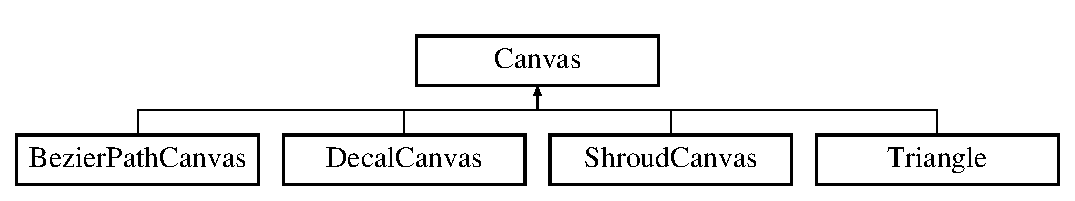
\includegraphics[height=2.000000cm]{class_canvas}
\end{center}
\end{figure}
\subsection*{Public Member Functions}
\begin{DoxyCompactItemize}
\item 
\hypertarget{class_canvas_a53b246273af5f8312e98963ebc5f18c8}{{\bfseries Canvas} (\hyperlink{class_target}{Target} $\ast$t, color\-\_\-t bg, \hyperlink{class_best_canvas}{Best\-Canvas} $\ast$bc)}\label{class_canvas_a53b246273af5f8312e98963ebc5f18c8}

\item 
\hypertarget{class_canvas_ae3d42b2fc30548f6c6bf7d269067e9c7}{{\bfseries Canvas} (\hyperlink{class_target}{Target} $\ast$t, color\-\_\-t bg\-\_\-\-Red, color\-\_\-t bg\-\_\-\-Green, color\-\_\-t bg\-\_\-\-Blue, \hyperlink{class_best_canvas}{Best\-Canvas} $\ast$bc)}\label{class_canvas_ae3d42b2fc30548f6c6bf7d269067e9c7}

\item 
virtual \hyperlink{class_canvas_a237c4549ad2e27c729cd1f71e89f0fd9}{$\sim$\-Canvas} ()
\item 
\hypertarget{class_canvas_aa6fd94baa21ffded183b4bf2375d9516}{void {\bfseries set\-R\-G\-B\-Data} (int offset, \hyperlink{struct_r_g_b}{R\-G\-B} pixel)}\label{class_canvas_aa6fd94baa21ffded183b4bf2375d9516}

\item 
\hypertarget{class_canvas_a9b47997839f63bda394c7385eac6f96e}{const int {\bfseries get\-Data\-Offset} (\hyperlink{struct_coord}{Coord} c)}\label{class_canvas_a9b47997839f63bda394c7385eac6f96e}

\item 
\hypertarget{class_canvas_ab1686ad837e67a4c93d7539d0d3d0151}{\hyperlink{struct_r_g_b}{R\-G\-B} {\bfseries get\-R\-G\-B\-Data} (int offset)}\label{class_canvas_ab1686ad837e67a4c93d7539d0d3d0151}

\item 
\hypertarget{class_canvas_a9e51f90be565cb3e5d683cdf83d67956}{bool {\bfseries inside\-Canvas} (\hyperlink{struct_coord}{Coord})}\label{class_canvas_a9e51f90be565cb3e5d683cdf83d67956}

\item 
\hypertarget{class_canvas_ae397083afa0345eec9c0e212903a6394}{\hyperlink{struct_coord}{Coord} {\bfseries rotate2\-D} (\hyperlink{struct_coord}{Coord} c, float dx, float dy, float theta)}\label{class_canvas_ae397083afa0345eec9c0e212903a6394}

\item 
\hypertarget{class_canvas_abbde1d2cfe76cb174828233e610b62ac}{virtual bool {\bfseries save\-Image} (char $\ast$filename)=0}\label{class_canvas_abbde1d2cfe76cb174828233e610b62ac}

\item 
\hypertarget{class_canvas_a20a5bfc766b35f031f87602a33d004b1}{bool {\bfseries save\-H\-S\-V\-Image} (char $\ast$filename)}\label{class_canvas_a20a5bfc766b35f031f87602a33d004b1}

\item 
\hypertarget{class_canvas_a0cd8a0f0e6a1b8bae854d93277926951}{bool {\bfseries save\-R\-G\-B\-Image} (char $\ast$filename)}\label{class_canvas_a0cd8a0f0e6a1b8bae854d93277926951}

\item 
\hypertarget{class_canvas_abd119da0a1dc1b24a45c8c45bd398732}{virtual void {\bfseries reset\-Canvas} ()=0}\label{class_canvas_abd119da0a1dc1b24a45c8c45bd398732}

\item 
\hypertarget{class_canvas_aa5c92419e72221fd67fae506419ec165}{virtual void {\bfseries paint\-Canvas} (vector$<$ float $>$)=0}\label{class_canvas_aa5c92419e72221fd67fae506419ec165}

\item 
\hypertarget{class_canvas_a23c0eb700982cfb7e8f468b51aa7adde}{int {\bfseries get\-Num\-Draw\-Nodes} ()}\label{class_canvas_a23c0eb700982cfb7e8f468b51aa7adde}

\item 
\hypertarget{class_canvas_a9a96d277519345b76e27349ca8d6421d}{virtual void {\bfseries compute\-Fitness} ()=0}\label{class_canvas_a9a96d277519345b76e27349ca8d6421d}

\item 
\hypertarget{class_canvas_a21fb2ed04cb521a5cdb3516bfa7bf6f1}{virtual float {\bfseries get\-Fitness} ()=0}\label{class_canvas_a21fb2ed04cb521a5cdb3516bfa7bf6f1}

\item 
\hypertarget{class_canvas_af78dc240a3278b5d7abad1cd743e31c4}{const int {\bfseries get\-Size} ()}\label{class_canvas_af78dc240a3278b5d7abad1cd743e31c4}

\item 
\hypertarget{class_canvas_a32c661c9bf432d32b6b75d097cba614f}{bool {\bfseries pixel\-Is\-Dirty} (\hyperlink{struct_coord}{Coord} c)}\label{class_canvas_a32c661c9bf432d32b6b75d097cba614f}

\item 
\hypertarget{class_canvas_aff7ccbf887a62cfaf2785845d5dabb17}{bool {\bfseries pixel\-Is\-White} (\hyperlink{struct_coord}{Coord} c)}\label{class_canvas_aff7ccbf887a62cfaf2785845d5dabb17}

\item 
\hypertarget{class_canvas_ac2032301cc13268992ecf3df85b73de0}{void {\bfseries update\-Best\-Canvas} ()}\label{class_canvas_ac2032301cc13268992ecf3df85b73de0}

\item 
\hypertarget{class_canvas_a36f33f02cee811e0d5a13e659eeb1f73}{const int {\bfseries get\-Width} ()}\label{class_canvas_a36f33f02cee811e0d5a13e659eeb1f73}

\item 
\hypertarget{class_canvas_a0b94a41db3014f125219155940437505}{const int {\bfseries get\-Height} ()}\label{class_canvas_a0b94a41db3014f125219155940437505}

\end{DoxyCompactItemize}
\subsection*{Protected Member Functions}
\begin{DoxyCompactItemize}
\item 
\hypertarget{class_canvas_a6740306cd9f07901b2bc31c2d4bbc3a3}{void {\bfseries reset\-Num\-Draw\-Nodes} ()}\label{class_canvas_a6740306cd9f07901b2bc31c2d4bbc3a3}

\item 
\hypertarget{class_canvas_a9381d59bc23a115890fda270eecc69f1}{void {\bfseries increment\-Lines} ()}\label{class_canvas_a9381d59bc23a115890fda270eecc69f1}

\item 
\hypertarget{class_canvas_a0227884bab636ac95308b239c99f3466}{void {\bfseries set\-Background} (color\-\_\-t bg)}\label{class_canvas_a0227884bab636ac95308b239c99f3466}

\item 
\hypertarget{class_canvas_abf204df96ee5233c09817245942a52f5}{void {\bfseries set\-Background\-\_\-\-Red} (color\-\_\-t bg)}\label{class_canvas_abf204df96ee5233c09817245942a52f5}

\item 
\hypertarget{class_canvas_aacbfeb32c1611636b937d9eddc6042f0}{void {\bfseries set\-Background\-\_\-\-Green} (color\-\_\-t bg)}\label{class_canvas_aacbfeb32c1611636b937d9eddc6042f0}

\item 
\hypertarget{class_canvas_a447151f796bafcbd3cbbc5191d98aa40}{void {\bfseries set\-Background\-\_\-\-Blue} (color\-\_\-t bg)}\label{class_canvas_a447151f796bafcbd3cbbc5191d98aa40}

\item 
\hypertarget{class_canvas_a24ccd2a00993f23addb6b29080a9733a}{const color\-\_\-t {\bfseries get\-B\-G\-Color} ()}\label{class_canvas_a24ccd2a00993f23addb6b29080a9733a}

\item 
\hypertarget{class_canvas_a71cfe236e024ae60ac8941cca8f1eb7a}{const color\-\_\-t {\bfseries getbg\-Color\-\_\-\-Red} ()}\label{class_canvas_a71cfe236e024ae60ac8941cca8f1eb7a}

\item 
\hypertarget{class_canvas_a8d10f424606d7ac03bdb1197bd23742c}{const color\-\_\-t {\bfseries getbg\-Color\-\_\-\-Green} ()}\label{class_canvas_a8d10f424606d7ac03bdb1197bd23742c}

\item 
\hypertarget{class_canvas_a62e8cb7b9c0a99b64adda7ff5330e5a2}{const color\-\_\-t {\bfseries getbg\-Color\-\_\-\-Blue} ()}\label{class_canvas_a62e8cb7b9c0a99b64adda7ff5330e5a2}

\item 
\hypertarget{class_canvas_a2b7899e3b8ff4d9938b1b385011ccb25}{\hyperlink{class_target}{Target} $\ast$ {\bfseries get\-Target} ()}\label{class_canvas_a2b7899e3b8ff4d9938b1b385011ccb25}

\item 
\hypertarget{class_canvas_acb06d2e4116994f32121333e69585249}{\hyperlink{struct_h_s_v}{H\-S\-V} {\bfseries get\-H\-S\-V\-Data} (int offset)}\label{class_canvas_acb06d2e4116994f32121333e69585249}

\item 
\hypertarget{class_canvas_a7fba7a894a1857c9ee2fe34441629d52}{void {\bfseries set\-H\-S\-V\-Data} (int offset, \hyperlink{struct_h_s_v}{H\-S\-V} pixel)}\label{class_canvas_a7fba7a894a1857c9ee2fe34441629d52}

\item 
\hypertarget{class_canvas_a8a7184ebaa6704048362972407787a59}{void {\bfseries set\-H\-S\-V\-Fitness\-H} (float f)}\label{class_canvas_a8a7184ebaa6704048362972407787a59}

\item 
\hypertarget{class_canvas_aa4e1c90061a6814daf5bbca65e1e398a}{void {\bfseries set\-H\-S\-V\-Fitness\-S} (float f)}\label{class_canvas_aa4e1c90061a6814daf5bbca65e1e398a}

\item 
\hypertarget{class_canvas_a068052d242a5c21a89b334224a127d19}{void {\bfseries set\-H\-S\-V\-Fitness\-V} (float f)}\label{class_canvas_a068052d242a5c21a89b334224a127d19}

\item 
\hypertarget{class_canvas_aa0c60ed66fcea208c32a2e3c8bf28923}{int {\bfseries degrees\-Of\-Separation} (int, int)}\label{class_canvas_aa0c60ed66fcea208c32a2e3c8bf28923}

\item 
\hypertarget{class_canvas_a56ba128080bcc03c8bb8b7d6c2cc9821}{void {\bfseries print\-Color} (\hyperlink{struct_r_g_b}{R\-G\-B} color)}\label{class_canvas_a56ba128080bcc03c8bb8b7d6c2cc9821}

\item 
\hypertarget{class_canvas_a570498c742d3e171b7be1c498f0e75f1}{void {\bfseries print\-Color} (\hyperlink{struct_h_s_v}{H\-S\-V} color)}\label{class_canvas_a570498c742d3e171b7be1c498f0e75f1}

\item 
\hypertarget{class_canvas_a95ecf73c2b84c001d12bc6dc6940091e}{\hyperlink{struct_r_g_b}{R\-G\-B} {\bfseries target\-Pixel\-R\-G\-B} (\hyperlink{struct_coord}{Coord} c)}\label{class_canvas_a95ecf73c2b84c001d12bc6dc6940091e}

\item 
\hypertarget{class_canvas_a04b66e5e405d8785984a01d7b8dc639c}{\hyperlink{struct_h_s_v}{H\-S\-V} {\bfseries target\-Pixel\-H\-S\-V} (\hyperlink{struct_coord}{Coord} c)}\label{class_canvas_a04b66e5e405d8785984a01d7b8dc639c}

\item 
\hypertarget{class_canvas_aa8c5064fd62e3aa1fde2bf94b806281e}{int {\bfseries target\-Hue} (\hyperlink{struct_coord}{Coord} c)}\label{class_canvas_aa8c5064fd62e3aa1fde2bf94b806281e}

\item 
\hypertarget{class_canvas_aca87eeb2759686e9f9d1f28d9716393a}{int {\bfseries target\-Sat} (\hyperlink{struct_coord}{Coord} c)}\label{class_canvas_aca87eeb2759686e9f9d1f28d9716393a}

\item 
\hypertarget{class_canvas_a69e2bd44307edae0ac346fefb80be422}{int {\bfseries target\-Val} (\hyperlink{struct_coord}{Coord} c)}\label{class_canvas_a69e2bd44307edae0ac346fefb80be422}

\item 
\hypertarget{class_canvas_a13059f62106ec98aa56042e053a9d00a}{int {\bfseries target\-Sat\-Gradient} (\hyperlink{struct_coord}{Coord} c)}\label{class_canvas_a13059f62106ec98aa56042e053a9d00a}

\item 
\hypertarget{class_canvas_a6f9d4ad8953ce2e7294e7ef611dcc7da}{int {\bfseries target\-Val\-Gradient} (\hyperlink{struct_coord}{Coord} c)}\label{class_canvas_a6f9d4ad8953ce2e7294e7ef611dcc7da}

\item 
\hypertarget{class_canvas_a70268f85eead1127cffba07515ebc777}{float {\bfseries target\-Sat\-Direction} (\hyperlink{struct_coord}{Coord} c)}\label{class_canvas_a70268f85eead1127cffba07515ebc777}

\item 
\hypertarget{class_canvas_ab8fe4798eaa8d2f630622b0a92664c25}{float {\bfseries target\-Val\-Direction} (\hyperlink{struct_coord}{Coord} c)}\label{class_canvas_ab8fe4798eaa8d2f630622b0a92664c25}

\item 
\hypertarget{class_canvas_a467ca92f410dfb513f0cb6ab6fddcb9b}{int {\bfseries match\-Hue} (\hyperlink{struct_coord}{Coord} c, int h)}\label{class_canvas_a467ca92f410dfb513f0cb6ab6fddcb9b}

\item 
\hypertarget{class_canvas_a51a62303ba86699a047c9b82151cc851}{int {\bfseries match\-Sat} (\hyperlink{struct_coord}{Coord} c, int s)}\label{class_canvas_a51a62303ba86699a047c9b82151cc851}

\item 
\hypertarget{class_canvas_ab6c6ee4bb92793b61b4c99b64e3e4514}{int {\bfseries match\-Val} (\hyperlink{struct_coord}{Coord} c, int v)}\label{class_canvas_ab6c6ee4bb92793b61b4c99b64e3e4514}

\item 
\hypertarget{class_canvas_a25fc15e87b8526fd411e227bfe94d1ca}{void {\bfseries compute\-H\-S\-V\-Fitness} ()}\label{class_canvas_a25fc15e87b8526fd411e227bfe94d1ca}

\end{DoxyCompactItemize}
\subsection*{Protected Attributes}
\begin{DoxyCompactItemize}
\item 
\hypertarget{class_canvas_a93c8956f408b11c81073f5d748a8e3b3}{\hyperlink{class_best_canvas}{Best\-Canvas} $\ast$ {\bfseries best\-Canvas}}\label{class_canvas_a93c8956f408b11c81073f5d748a8e3b3}

\item 
\hypertarget{class_canvas_aeff1549bc9fb9469f68227dbbee4a4de}{float {\bfseries hsv\-Fitness\-H}}\label{class_canvas_aeff1549bc9fb9469f68227dbbee4a4de}

\item 
\hypertarget{class_canvas_af04ba6d3e079fa937575f7ef80bfac6d}{float {\bfseries hsv\-Fitness\-S}}\label{class_canvas_af04ba6d3e079fa937575f7ef80bfac6d}

\item 
\hypertarget{class_canvas_a16bfdb1b384498d5aa0cbd674c6abfe4}{float {\bfseries hsv\-Fitness\-V}}\label{class_canvas_a16bfdb1b384498d5aa0cbd674c6abfe4}

\end{DoxyCompactItemize}


\subsection{Constructor \& Destructor Documentation}
\hypertarget{class_canvas_a237c4549ad2e27c729cd1f71e89f0fd9}{\index{Canvas@{Canvas}!$\sim$\-Canvas@{$\sim$\-Canvas}}
\index{$\sim$\-Canvas@{$\sim$\-Canvas}!Canvas@{Canvas}}
\subsubsection[{$\sim$\-Canvas}]{\setlength{\rightskip}{0pt plus 5cm}Canvas\-::$\sim$\-Canvas (
\begin{DoxyParamCaption}
{}
\end{DoxyParamCaption}
)\hspace{0.3cm}{\ttfamily [virtual]}}}\label{class_canvas_a237c4549ad2e27c729cd1f71e89f0fd9}
Canvas\-::\-Canvas() \{ \} 

The documentation for this class was generated from the following files\-:\begin{DoxyCompactItemize}
\item 
Canvas.\-h\item 
Canvas.\-cpp\end{DoxyCompactItemize}

\hypertarget{class_color_converter}{\section{Color\-Converter Class Reference}
\label{class_color_converter}\index{Color\-Converter@{Color\-Converter}}
}
\subsection*{Public Member Functions}
\begin{DoxyCompactItemize}
\item 
\hypertarget{class_color_converter_aa9abd3937e87e0fcb712d2ca7a611402}{color\-\_\-t {\bfseries rgb2gray} (\hyperlink{struct_r_g_b}{R\-G\-B})}\label{class_color_converter_aa9abd3937e87e0fcb712d2ca7a611402}

\item 
\hypertarget{class_color_converter_a351341558ba62951aefd6d3d9bf09785}{\hyperlink{struct_h_s_v}{H\-S\-V} {\bfseries rgb2hsv} (\hyperlink{struct_r_g_b}{R\-G\-B})}\label{class_color_converter_a351341558ba62951aefd6d3d9bf09785}

\item 
\hypertarget{class_color_converter_aca4539e968906df8d1ecd102464a0372}{\hyperlink{struct_r_g_b}{R\-G\-B} {\bfseries hsv2rgb} (\hyperlink{struct_h_s_v}{H\-S\-V})}\label{class_color_converter_aca4539e968906df8d1ecd102464a0372}

\item 
\hypertarget{class_color_converter_a43a52a206fb9f246d31af8f7e39b4110}{\hyperlink{struct_r_g_b}{R\-G\-B} {\bfseries hex2rgb} (std\-::string)}\label{class_color_converter_a43a52a206fb9f246d31af8f7e39b4110}

\item 
\hypertarget{class_color_converter_adb9a22672900e507c63b172a14713e95}{int {\bfseries round\-Off} (float, int)}\label{class_color_converter_adb9a22672900e507c63b172a14713e95}

\end{DoxyCompactItemize}


The documentation for this class was generated from the following files\-:\begin{DoxyCompactItemize}
\item 
Color\-Converter.\-h\item 
Color\-Converter.\-cpp\end{DoxyCompactItemize}

\hypertarget{class_config_reader}{\section{Config\-Reader Class Reference}
\label{class_config_reader}\index{Config\-Reader@{Config\-Reader}}
}
\subsection*{Public Member Functions}
\begin{DoxyCompactItemize}
\item 
\hypertarget{class_config_reader_aa525c738a01392f1fa61b05a2f16063a}{void {\bfseries read\-Painter\-Data} ()}\label{class_config_reader_aa525c738a01392f1fa61b05a2f16063a}

\item 
\hypertarget{class_config_reader_ad2c2a7bfc19b76357dc91d9def4c7992}{int {\bfseries get\-Population} ()}\label{class_config_reader_ad2c2a7bfc19b76357dc91d9def4c7992}

\item 
\hypertarget{class_config_reader_a5c2411ee0c0677015b9655dc7360c97e}{int {\bfseries get\-Initial\-Population} ()}\label{class_config_reader_a5c2411ee0c0677015b9655dc7360c97e}

\item 
\hypertarget{class_config_reader_a50cb73d4e053df9a16c16a6a650da147}{int {\bfseries get\-Generations} ()}\label{class_config_reader_a50cb73d4e053df9a16c16a6a650da147}

\item 
\hypertarget{class_config_reader_aaf6399eb399499490eae48fe29fe99eb}{int {\bfseries get\-Elitism} ()}\label{class_config_reader_aaf6399eb399499490eae48fe29fe99eb}

\item 
\hypertarget{class_config_reader_a9bb987d15fa1f2d13f7ada58e03e0a43}{int {\bfseries get\-Mutation} ()}\label{class_config_reader_a9bb987d15fa1f2d13f7ada58e03e0a43}

\item 
\hypertarget{class_config_reader_a1e2ade167d3e28489b4e2dc37242b8fd}{int {\bfseries get\-Crossover} ()}\label{class_config_reader_a1e2ade167d3e28489b4e2dc37242b8fd}

\item 
\hypertarget{class_config_reader_ae707de59f1e1c32bfa8f4961247758f6}{int {\bfseries get\-Max\-Tree} ()}\label{class_config_reader_ae707de59f1e1c32bfa8f4961247758f6}

\item 
\hypertarget{class_config_reader_ac8b0ed0d215cfbdb595f9ca91db0bc5c}{int {\bfseries get\-Min\-Tree} ()}\label{class_config_reader_ac8b0ed0d215cfbdb595f9ca91db0bc5c}

\item 
\hypertarget{class_config_reader_a48f25599934dd6a80694e312139d7fa8}{bool {\bfseries get\-Fuzzy\-Edges} ()}\label{class_config_reader_a48f25599934dd6a80694e312139d7fa8}

\item 
\hypertarget{class_config_reader_abc7d4bab01a5e1eeabb30e185a230455}{int {\bfseries get\-Sat\-Canny\-Lo} ()}\label{class_config_reader_abc7d4bab01a5e1eeabb30e185a230455}

\item 
\hypertarget{class_config_reader_ad275c15d54c720a54cd4010b5dc6a193}{int {\bfseries get\-Sat\-Canny\-Hi} ()}\label{class_config_reader_ad275c15d54c720a54cd4010b5dc6a193}

\item 
\hypertarget{class_config_reader_aecef166e19340044e96cc9aa033c2b0b}{int {\bfseries get\-Val\-Canny\-Lo} ()}\label{class_config_reader_aecef166e19340044e96cc9aa033c2b0b}

\item 
\hypertarget{class_config_reader_a5cc8adc5919047dfc7794a1ade63d031}{int {\bfseries get\-Val\-Canny\-Hi} ()}\label{class_config_reader_a5cc8adc5919047dfc7794a1ade63d031}

\item 
\hypertarget{class_config_reader_a825c0cdf7ac8c8698982d45730c656c8}{float {\bfseries get\-Fitness\-Target} ()}\label{class_config_reader_a825c0cdf7ac8c8698982d45730c656c8}

\item 
\hypertarget{class_config_reader_a3f399e2dc3622639d9fecff36e9951d2}{int {\bfseries get\-Random\-Seed} ()}\label{class_config_reader_a3f399e2dc3622639d9fecff36e9951d2}

\item 
\hypertarget{class_config_reader_ab7c21d8d74d01907e4ef64f2033bcaba}{int {\bfseries get\-Canvas\-B\-G} ()}\label{class_config_reader_ab7c21d8d74d01907e4ef64f2033bcaba}

\item 
\hypertarget{class_config_reader_af10edf0066b89aeb465f80b869c6b1e3}{int {\bfseries get\-Canvas\-B\-G\-\_\-\-Red} ()}\label{class_config_reader_af10edf0066b89aeb465f80b869c6b1e3}

\item 
\hypertarget{class_config_reader_a206a96e4b64d12105e36ef9ad98bf4ff}{int {\bfseries get\-Canvas\-B\-G\-\_\-\-Green} ()}\label{class_config_reader_a206a96e4b64d12105e36ef9ad98bf4ff}

\item 
\hypertarget{class_config_reader_a61718c31162418d22f3119bfc9d43f75}{int {\bfseries get\-Canvas\-B\-G\-\_\-\-Blue} ()}\label{class_config_reader_a61718c31162418d22f3119bfc9d43f75}

\item 
\hypertarget{class_config_reader_aa0093d6cc78780960771c5abd12937a1}{int {\bfseries get\-Colour\-Updater} ()}\label{class_config_reader_aa0093d6cc78780960771c5abd12937a1}

\item 
\hypertarget{class_config_reader_ae408fab7b0a2a214621f02d0c019a4e7}{int {\bfseries get\-Colour\-Mode} ()}\label{class_config_reader_ae408fab7b0a2a214621f02d0c019a4e7}

\item 
\hypertarget{class_config_reader_af337f0c19e0ed70d586a7471fc0b2d5e}{int {\bfseries get\-First\-Line\-Length} ()}\label{class_config_reader_af337f0c19e0ed70d586a7471fc0b2d5e}

\item 
\hypertarget{class_config_reader_a5f2b66c0fecfb1c542c68c3f89d4361f}{int {\bfseries get\-Second\-Line\-Length} ()}\label{class_config_reader_a5f2b66c0fecfb1c542c68c3f89d4361f}

\item 
\hypertarget{class_config_reader_a151c30e6eafab6be5d0f7f86659508bf}{int {\bfseries get\-Shape} ()}\label{class_config_reader_a151c30e6eafab6be5d0f7f86659508bf}

\item 
\hypertarget{class_config_reader_a09ef925e405ebd002bbe61c554020dcc}{int {\bfseries get\-Type\-Triangle} ()}\label{class_config_reader_a09ef925e405ebd002bbe61c554020dcc}

\item 
\hypertarget{class_config_reader_a8f9d90b2ea2da85939040a41b1395260}{std\-::string {\bfseries get\-Custom\-Decal\-File\-Name} ()}\label{class_config_reader_a8f9d90b2ea2da85939040a41b1395260}

\item 
\hypertarget{class_config_reader_a6f42945c6aa5a1669ccd59c3f998b456}{std\-::string {\bfseries get\-Path\-To\-Target} ()}\label{class_config_reader_a6f42945c6aa5a1669ccd59c3f998b456}

\item 
\hypertarget{class_config_reader_a44d2bef5c4bc3d42ff4d5e1a6d6dae4f}{std\-::string {\bfseries get\-Path\-To\-Mask} ()}\label{class_config_reader_a44d2bef5c4bc3d42ff4d5e1a6d6dae4f}

\item 
\hypertarget{class_config_reader_a9fe59626354c78f6e52f06ff98de38c6}{std\-::string {\bfseries get\-Path\-To\-Output} ()}\label{class_config_reader_a9fe59626354c78f6e52f06ff98de38c6}

\item 
\hypertarget{class_config_reader_a90abd02c164c974d5c67577ee29c1c54}{std\-::string {\bfseries get\-Path\-To\-Palette} ()}\label{class_config_reader_a90abd02c164c974d5c67577ee29c1c54}

\item 
\hypertarget{class_config_reader_acc7926f146161c7512631296c6169c27}{std\-::string {\bfseries get\-Target\-File\-Name} ()}\label{class_config_reader_acc7926f146161c7512631296c6169c27}

\item 
\hypertarget{class_config_reader_ac130d7d879988452891fc1f4d5e89b1a}{std\-::string {\bfseries get\-Palette} ()}\label{class_config_reader_ac130d7d879988452891fc1f4d5e89b1a}

\item 
\hypertarget{class_config_reader_a80d01e04ca22ca126bbdbc476984cfea}{std\-::string {\bfseries get\-Version} ()}\label{class_config_reader_a80d01e04ca22ca126bbdbc476984cfea}

\item 
\hypertarget{class_config_reader_a5a2e68a5fb89b5d0bb2b8d38150edcd1}{bool {\bfseries get\-Line\-Art\-Thickness} ()}\label{class_config_reader_a5a2e68a5fb89b5d0bb2b8d38150edcd1}

\item 
\hypertarget{class_config_reader_ab4f64f1b863a6d78ef8087d1d41c6889}{int {\bfseries get\-Draw\-Mode} ()}\label{class_config_reader_ab4f64f1b863a6d78ef8087d1d41c6889}

\item 
\hypertarget{class_config_reader_a813f80a6afee19bdfd1787db5c277676}{double {\bfseries get\-Fitness\-Render\-Threshold} ()}\label{class_config_reader_a813f80a6afee19bdfd1787db5c277676}

\item 
\hypertarget{class_config_reader_abe4991a967a948f5bfa7d61eca9e26c2}{bool {\bfseries get\-Prog2} ()}\label{class_config_reader_abe4991a967a948f5bfa7d61eca9e26c2}

\item 
\hypertarget{class_config_reader_a15c4ba819559d15420c43c40b455972a}{bool {\bfseries get\-Prog3} ()}\label{class_config_reader_a15c4ba819559d15420c43c40b455972a}

\item 
\hypertarget{class_config_reader_a73b004a202d836b0f5947675529dbb4c}{bool {\bfseries get\-Prog4} ()}\label{class_config_reader_a73b004a202d836b0f5947675529dbb4c}

\item 
\hypertarget{class_config_reader_ac33a1ec754771eb38d945e312493fc70}{bool {\bfseries get\-Using\-Adaptive\-Canvas} ()}\label{class_config_reader_ac33a1ec754771eb38d945e312493fc70}

\item 
\hypertarget{class_config_reader_ad2722e1f259e6a4e46b5dc0166fdf80d}{bool {\bfseries get\-Fast\-Shroud} ()}\label{class_config_reader_ad2722e1f259e6a4e46b5dc0166fdf80d}

\item 
\hypertarget{class_config_reader_a16ec9fa2175b2c7f28253ca3ec05c2da}{int {\bfseries get\-Line\-Art\-Color\-Mode} ()}\label{class_config_reader_a16ec9fa2175b2c7f28253ca3ec05c2da}

\item 
\hypertarget{class_config_reader_a8b50213030f7964d77e8989f8ee6c5e4}{int {\bfseries get\-Shroud\-Pixel\-Strategy} ()}\label{class_config_reader_a8b50213030f7964d77e8989f8ee6c5e4}

\item 
\hypertarget{class_config_reader_ac48c38cb4fd2d04c7761b4813d94cd90}{int {\bfseries get\-Tournament\-Size} ()}\label{class_config_reader_ac48c38cb4fd2d04c7761b4813d94cd90}

\item 
\hypertarget{class_config_reader_aaf1d7c03b3b4b3e71e12e6161b09db34}{void {\bfseries set\-Shroud\-Log\-Name} (char $\ast$newlog\-File\-Name)}\label{class_config_reader_aaf1d7c03b3b4b3e71e12e6161b09db34}

\item 
\hypertarget{class_config_reader_ac5df2afab92273c5a69c61fb8ffc9355}{char $\ast$ {\bfseries get\-Shroud\-Log\-Name} ()}\label{class_config_reader_ac5df2afab92273c5a69c61fb8ffc9355}

\item 
\hypertarget{class_config_reader_a7bf5f509fd6103cf351c384ddde32149}{void {\bfseries set\-Error\-Log\-Bad} (bool newflag)}\label{class_config_reader_a7bf5f509fd6103cf351c384ddde32149}

\item 
\hypertarget{class_config_reader_a5b5baa8c5865fd75f87d3fe69dc2f814}{string {\bfseries get\-Error\-Log\-Bad} ()}\label{class_config_reader_a5b5baa8c5865fd75f87d3fe69dc2f814}

\end{DoxyCompactItemize}
\subsection*{Public Attributes}
\begin{DoxyCompactItemize}
\item 
\hypertarget{class_config_reader_adff3f922c1af68d2ff3ffb2935f9ff7b}{char $\ast$ {\bfseries log\-File\-Name}}\label{class_config_reader_adff3f922c1af68d2ff3ffb2935f9ff7b}

\item 
\hypertarget{class_config_reader_abab3606d626f5ae659ffd34a6ecab8c2}{bool {\bfseries flag}}\label{class_config_reader_abab3606d626f5ae659ffd34a6ecab8c2}

\item 
\hypertarget{class_config_reader_a1ab9194bdcf3d05cddc5ddcfe99dc08f}{int {\bfseries current\-Genereation}}\label{class_config_reader_a1ab9194bdcf3d05cddc5ddcfe99dc08f}

\end{DoxyCompactItemize}
\subsection*{Static Public Attributes}
\begin{DoxyCompactItemize}
\item 
\hypertarget{class_config_reader_a728af86620d2f7bd22f8f50dc576dfbc}{static const int {\bfseries D\-R\-A\-W\-\_\-\-M\-O\-D\-E\-\_\-\-S\-H\-R\-O\-U\-D} = 0}\label{class_config_reader_a728af86620d2f7bd22f8f50dc576dfbc}

\item 
\hypertarget{class_config_reader_af7fb8fa1f2cc76913afc78a2726e44a6}{static const int {\bfseries D\-R\-A\-W\-\_\-\-M\-O\-D\-E\-\_\-\-D\-E\-C\-A\-L\-S} = 1}\label{class_config_reader_af7fb8fa1f2cc76913afc78a2726e44a6}

\item 
\hypertarget{class_config_reader_a51777b70066b67ddb71b1f2a0762e20a}{static const int {\bfseries D\-R\-A\-W\-\_\-\-M\-O\-D\-E\-\_\-\-S\-Q\-U\-I\-G\-G\-L\-E} = 2}\label{class_config_reader_a51777b70066b67ddb71b1f2a0762e20a}

\end{DoxyCompactItemize}


The documentation for this class was generated from the following files\-:\begin{DoxyCompactItemize}
\item 
Config\-Reader.\-h\item 
Config\-Reader.\-cpp\end{DoxyCompactItemize}

\hypertarget{struct_coord}{\section{Coord Struct Reference}
\label{struct_coord}\index{Coord@{Coord}}
}
\subsection*{Public Attributes}
\begin{DoxyCompactItemize}
\item 
\hypertarget{struct_coord_a089b098faaca481f53834c7cd7605da5}{float {\bfseries x}}\label{struct_coord_a089b098faaca481f53834c7cd7605da5}

\item 
\hypertarget{struct_coord_a55a67a26b632758699c9f999348d9f06}{float {\bfseries y}}\label{struct_coord_a55a67a26b632758699c9f999348d9f06}

\end{DoxyCompactItemize}


The documentation for this struct was generated from the following file\-:\begin{DoxyCompactItemize}
\item 
Utility.\-h\end{DoxyCompactItemize}

\hypertarget{class_decal}{\section{Decal Class Reference}
\label{class_decal}\index{Decal@{Decal}}
}
\subsection*{Public Member Functions}
\begin{DoxyCompactItemize}
\item 
\hypertarget{class_decal_a101d637231bbe15438573ff44481e025}{{\bfseries Decal} (\hyperlink{class_config_reader}{Config\-Reader} $\ast$reader, int min\-Dim, int max\-Dim)}\label{class_decal_a101d637231bbe15438573ff44481e025}

\item 
\hypertarget{class_decal_aca34cd0f099e08c77d5309eb1177b6db}{void {\bfseries set\-Location} (float f1, float f2)}\label{class_decal_aca34cd0f099e08c77d5309eb1177b6db}

\item 
\hypertarget{class_decal_ad59c6e4cfb8b06e7403aaf7a12a96ba8}{void {\bfseries set\-Color} (float f1, float f2, float f3)}\label{class_decal_ad59c6e4cfb8b06e7403aaf7a12a96ba8}

\item 
\hypertarget{class_decal_a4b3153696a223ec85c53e22876023a14}{void {\bfseries set\-Color} (\hyperlink{struct_h_s_v}{H\-S\-V} col)}\label{class_decal_a4b3153696a223ec85c53e22876023a14}

\item 
\hypertarget{class_decal_abcf93a8a28597b3e07ca8268af2ef049}{\hyperlink{struct_coord}{Coord} {\bfseries get\-Location} ()}\label{class_decal_abcf93a8a28597b3e07ca8268af2ef049}

\item 
\hypertarget{class_decal_a88024aec965f854e6ee74867b107963c}{\hyperlink{struct_r_g_b}{R\-G\-B} {\bfseries get\-R\-G\-B} ()}\label{class_decal_a88024aec965f854e6ee74867b107963c}

\item 
\hypertarget{class_decal_a78513a5e1b703ae65933f20f45cf8011}{\hyperlink{struct_h_s_v}{H\-S\-V} {\bfseries get\-H\-S\-V} ()}\label{class_decal_a78513a5e1b703ae65933f20f45cf8011}

\item 
\hypertarget{class_decal_a7d789f497a9019c4ab1fc2377038fc32}{int {\bfseries get\-Draw\-Length} ()}\label{class_decal_a7d789f497a9019c4ab1fc2377038fc32}

\item 
\hypertarget{class_decal_ad25e74f9b24b4487713a64fd2b8711c0}{double {\bfseries get\-Stroke\-Angle} ()}\label{class_decal_ad25e74f9b24b4487713a64fd2b8711c0}

\item 
\hypertarget{class_decal_ab455f1768097265f73022194f2830861}{int {\bfseries get\-Decal\-Width} ()}\label{class_decal_ab455f1768097265f73022194f2830861}

\end{DoxyCompactItemize}


The documentation for this class was generated from the following files\-:\begin{DoxyCompactItemize}
\item 
Decal.\-h\item 
Decal.\-cpp\end{DoxyCompactItemize}

\hypertarget{class_decal_canvas}{\section{Decal\-Canvas Class Reference}
\label{class_decal_canvas}\index{Decal\-Canvas@{Decal\-Canvas}}
}
Inheritance diagram for Decal\-Canvas\-:\begin{figure}[H]
\begin{center}
\leavevmode
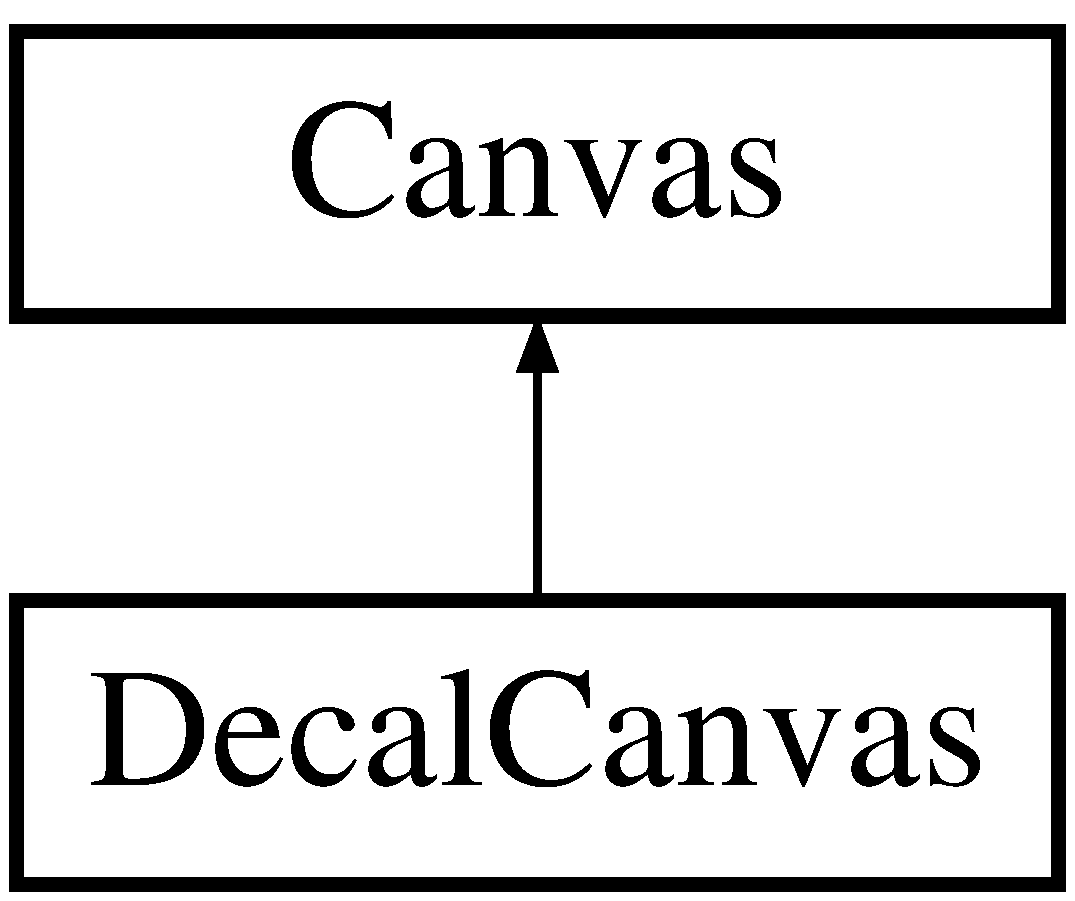
\includegraphics[height=2.000000cm]{class_decal_canvas}
\end{center}
\end{figure}
\subsection*{Public Member Functions}
\begin{DoxyCompactItemize}
\item 
\hypertarget{class_decal_canvas_ad00c8fbce88da1fd173f7da551f7ef95}{{\bfseries Decal\-Canvas} (\hyperlink{class_target}{Target} $\ast$t, color\-\_\-t bg, \hyperlink{class_best_canvas}{Best\-Canvas} $\ast$bc, \hyperlink{class_config_reader}{Config\-Reader} $\ast$reader)}\label{class_decal_canvas_ad00c8fbce88da1fd173f7da551f7ef95}

\item 
\hypertarget{class_decal_canvas_adbf1ef248c1cf7b6ed09abfa1ec05c08}{void {\bfseries paint\-Canvas} (vector$<$ float $>$)}\label{class_decal_canvas_adbf1ef248c1cf7b6ed09abfa1ec05c08}

\item 
\hypertarget{class_decal_canvas_a64baadb9a31c5aa598a45ce402d6d66a}{void {\bfseries reset\-Canvas} ()}\label{class_decal_canvas_a64baadb9a31c5aa598a45ce402d6d66a}

\item 
\hypertarget{class_decal_canvas_a8f122bff9c7696f184b8903dbb295af5}{\hyperlink{class_decal}{Decal} $\ast$ {\bfseries get\-Decal} ()}\label{class_decal_canvas_a8f122bff9c7696f184b8903dbb295af5}

\item 
\hypertarget{class_decal_canvas_aa2d4c9185e12bad6aa590a9f58477063}{void {\bfseries compute\-Stroke} ()}\label{class_decal_canvas_aa2d4c9185e12bad6aa590a9f58477063}

\item 
\hypertarget{class_decal_canvas_a6f9a66f4a1f22e227ef9120410534531}{void {\bfseries compute\-Fitness} ()}\label{class_decal_canvas_a6f9a66f4a1f22e227ef9120410534531}

\item 
\hypertarget{class_decal_canvas_a1e0134f001a92ce161838286fa73ad69}{float {\bfseries get\-Fitness} ()}\label{class_decal_canvas_a1e0134f001a92ce161838286fa73ad69}

\item 
\hypertarget{class_decal_canvas_a7309b13ba847f9efd36f94f50d2238bd}{bool {\bfseries save\-Image} (char $\ast$filename)}\label{class_decal_canvas_a7309b13ba847f9efd36f94f50d2238bd}

\end{DoxyCompactItemize}
\subsection*{Additional Inherited Members}


The documentation for this class was generated from the following files\-:\begin{DoxyCompactItemize}
\item 
Decal\-Canvas.\-h\item 
Decal\-Canvas.\-cpp\end{DoxyCompactItemize}

\hypertarget{class_draw2}{\section{Draw2 Class Reference}
\label{class_draw2}\index{Draw2@{Draw2}}
}
Inheritance diagram for Draw2\-:\begin{figure}[H]
\begin{center}
\leavevmode
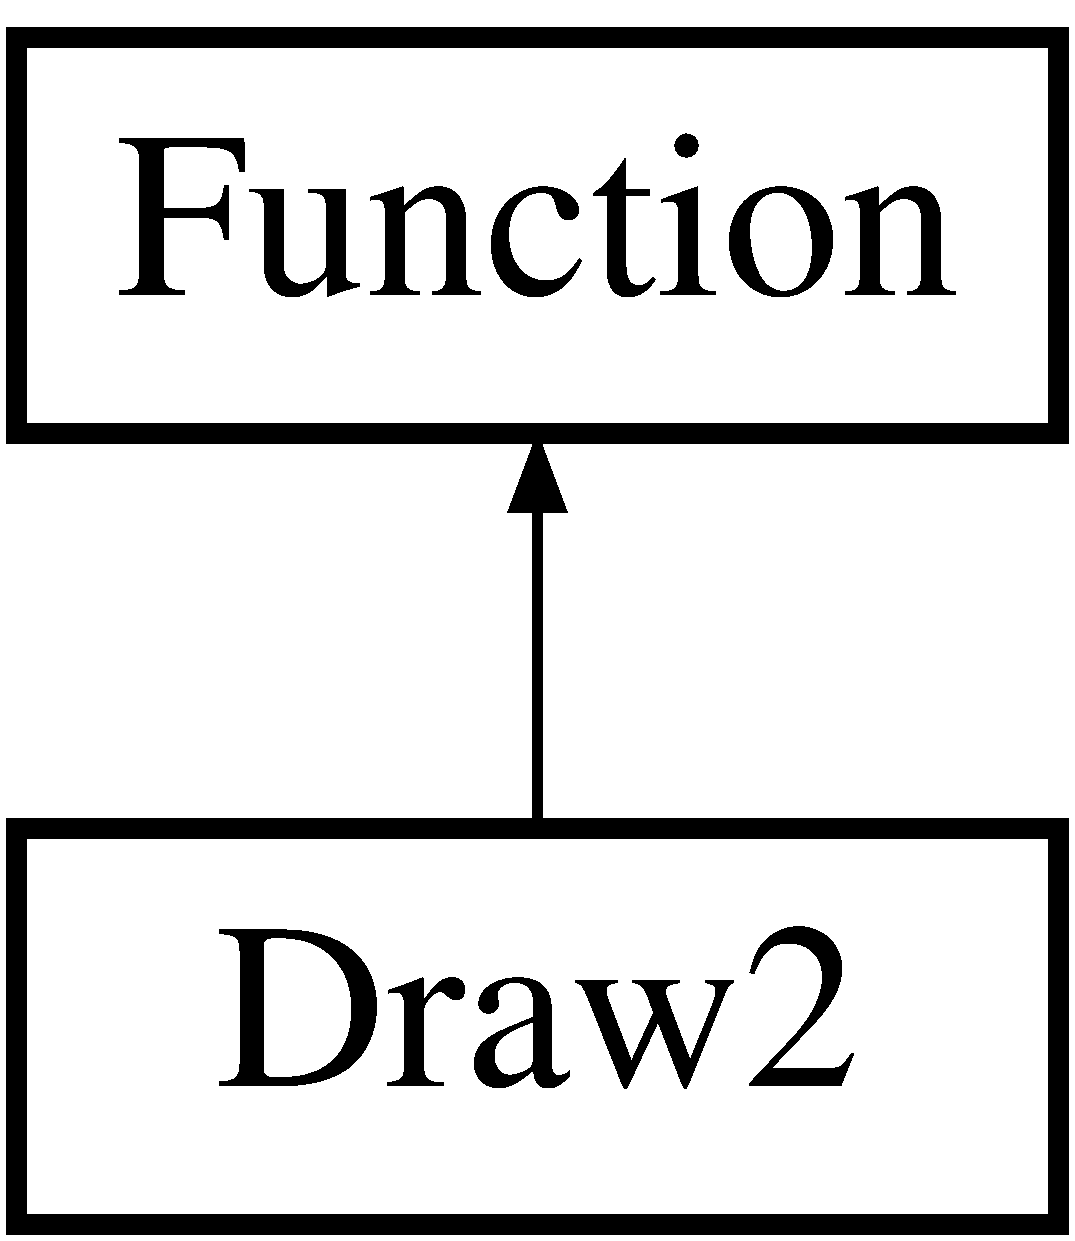
\includegraphics[height=2.000000cm]{class_draw2}
\end{center}
\end{figure}
\subsection*{Public Member Functions}
\begin{DoxyCompactItemize}
\item 
\hypertarget{class_draw2_a60ad134856f332bd4e3134eb3b0cef48}{{\bfseries Draw2} (G\-P\-Config $\ast$conf)}\label{class_draw2_a60ad134856f332bd4e3134eb3b0cef48}

\item 
\hypertarget{class_draw2_affe1fb09b91b328b5f9edf6a8e44995b}{virtual void {\bfseries evaluate} (Return\-Data $\ast$out)}\label{class_draw2_affe1fb09b91b328b5f9edf6a8e44995b}

\item 
\hypertarget{class_draw2_af82e7c3c4e46ad383ce3cb4a8589872d}{virtual Node $\ast$ {\bfseries copy} ()}\label{class_draw2_af82e7c3c4e46ad383ce3cb4a8589872d}

\end{DoxyCompactItemize}
\subsection*{Static Public Member Functions}
\begin{DoxyCompactItemize}
\item 
\hypertarget{class_draw2_acc0991ece5e007a9cca5d3f84c4f5bb4}{static Function $\ast$ {\bfseries generate} (const string \&name, G\-P\-Config $\ast$conf)}\label{class_draw2_acc0991ece5e007a9cca5d3f84c4f5bb4}

\end{DoxyCompactItemize}


The documentation for this class was generated from the following files\-:\begin{DoxyCompactItemize}
\item 
Draw2.\-h\item 
Draw2.\-cpp\end{DoxyCompactItemize}

\hypertarget{class_draw4}{\section{Draw4 Class Reference}
\label{class_draw4}\index{Draw4@{Draw4}}
}
Inheritance diagram for Draw4\-:\begin{figure}[H]
\begin{center}
\leavevmode
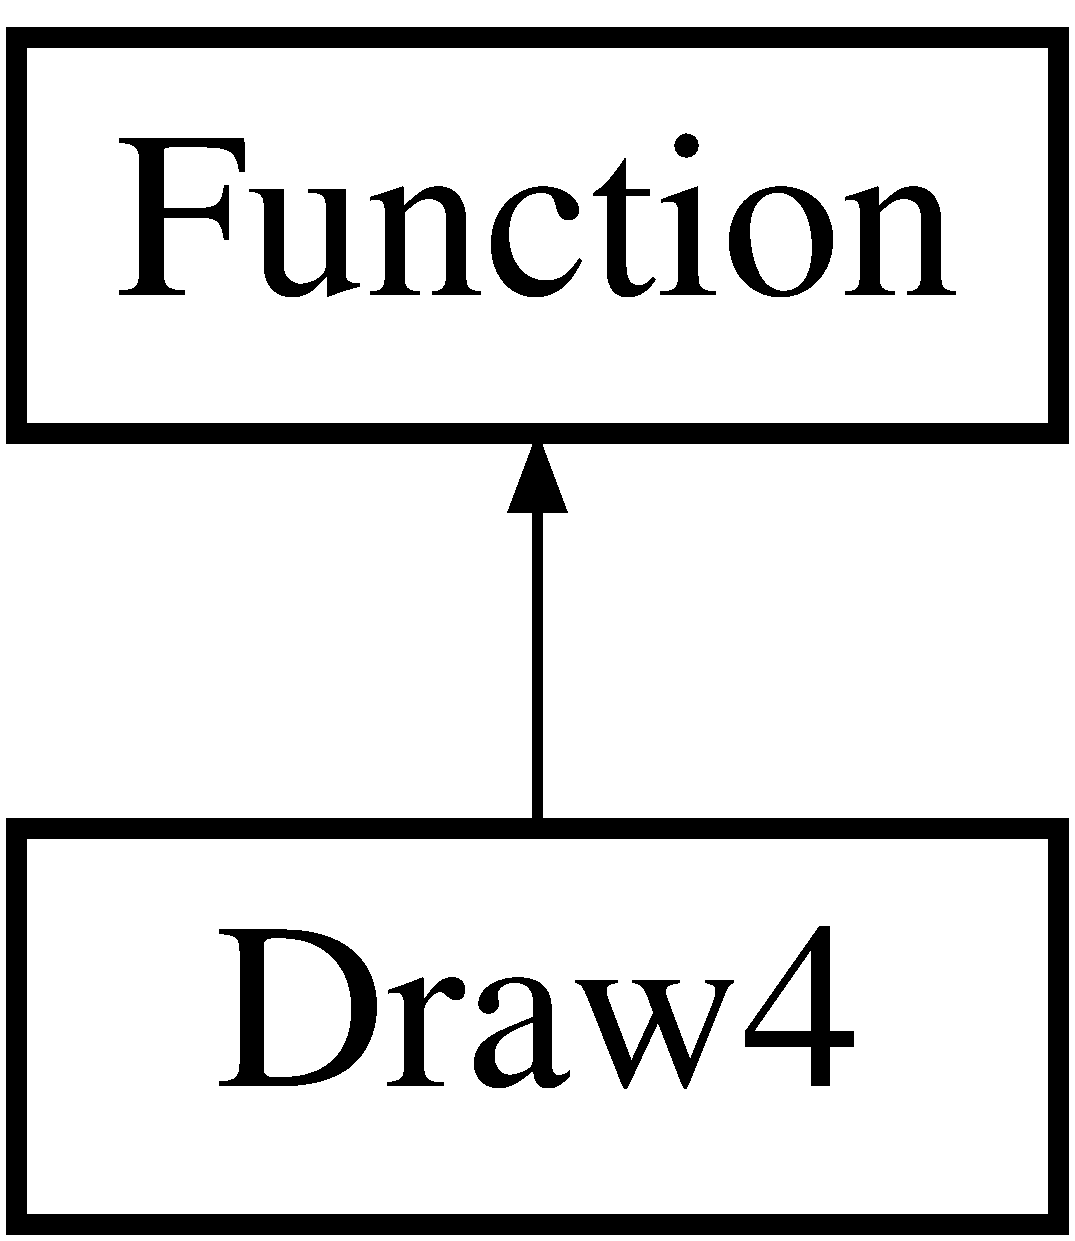
\includegraphics[height=2.000000cm]{class_draw4}
\end{center}
\end{figure}
\subsection*{Public Member Functions}
\begin{DoxyCompactItemize}
\item 
\hypertarget{class_draw4_a30a878a94519eb6c291629927d5edf5d}{{\bfseries Draw4} (G\-P\-Config $\ast$conf)}\label{class_draw4_a30a878a94519eb6c291629927d5edf5d}

\item 
\hypertarget{class_draw4_a2eeefbe82ec2b6fef14e8bd5947c02ac}{virtual void {\bfseries evaluate} (Return\-Data $\ast$out)}\label{class_draw4_a2eeefbe82ec2b6fef14e8bd5947c02ac}

\item 
\hypertarget{class_draw4_a6e4128cfa6b2b59dd08eb7e25da03f2e}{virtual Node $\ast$ {\bfseries copy} ()}\label{class_draw4_a6e4128cfa6b2b59dd08eb7e25da03f2e}

\end{DoxyCompactItemize}
\subsection*{Static Public Member Functions}
\begin{DoxyCompactItemize}
\item 
\hypertarget{class_draw4_a125086be4643dd452fc5f952a61f9e83}{static Function $\ast$ {\bfseries generate} (const string \&name, G\-P\-Config $\ast$conf)}\label{class_draw4_a125086be4643dd452fc5f952a61f9e83}

\end{DoxyCompactItemize}


The documentation for this class was generated from the following files\-:\begin{DoxyCompactItemize}
\item 
Draw4.\-h\item 
Draw4.\-cpp\end{DoxyCompactItemize}

\hypertarget{class_draw6}{\section{Draw6 Class Reference}
\label{class_draw6}\index{Draw6@{Draw6}}
}
Inheritance diagram for Draw6\-:\begin{figure}[H]
\begin{center}
\leavevmode
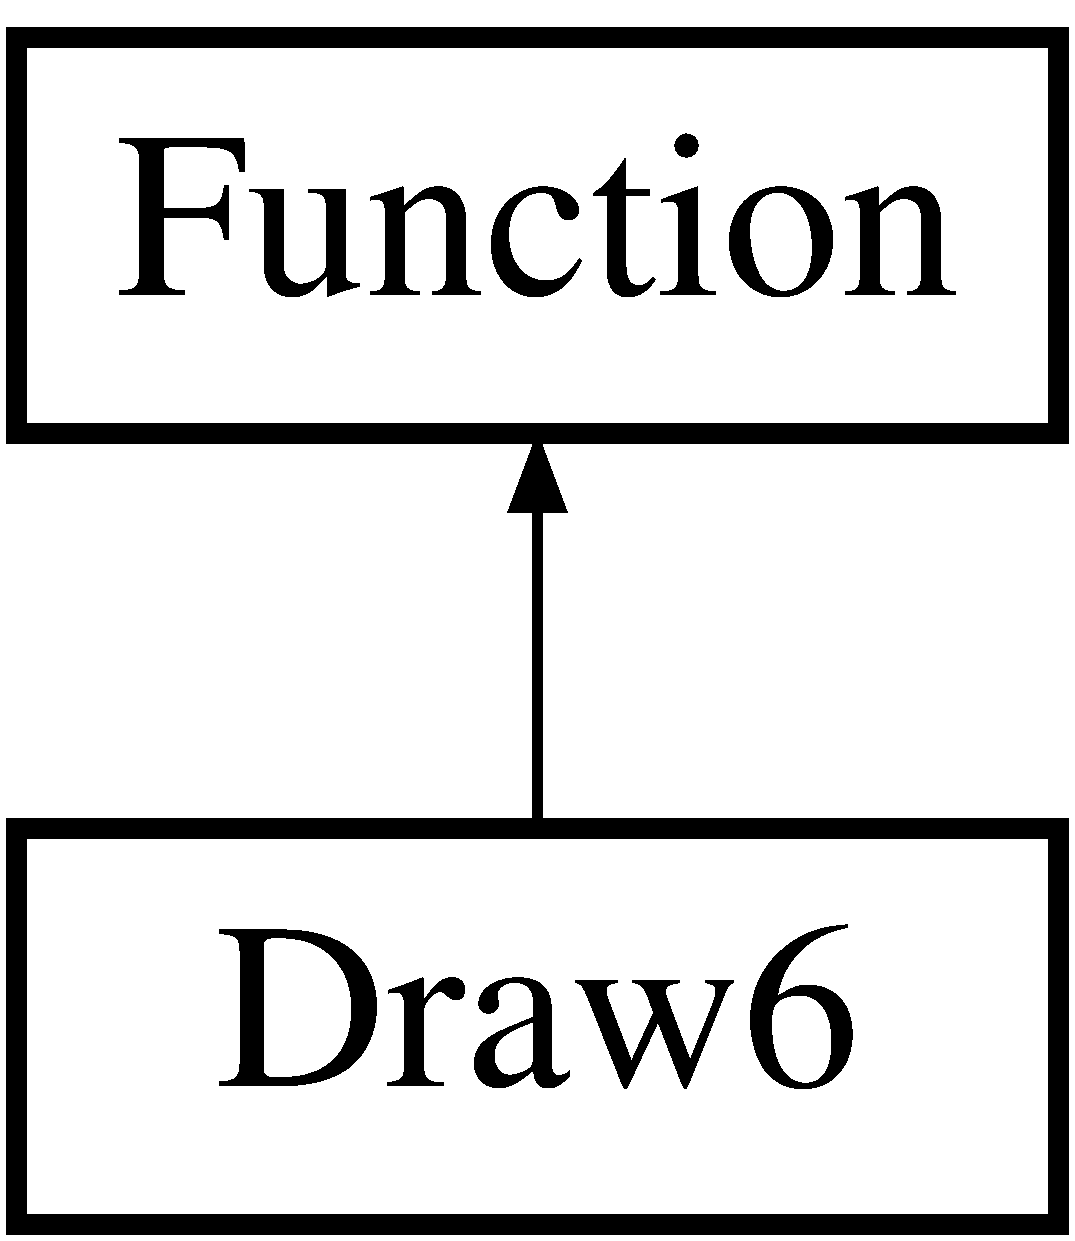
\includegraphics[height=2.000000cm]{class_draw6}
\end{center}
\end{figure}
\subsection*{Public Member Functions}
\begin{DoxyCompactItemize}
\item 
\hypertarget{class_draw6_a3ce8484795df7bd08600ee8a7d457852}{{\bfseries Draw6} (G\-P\-Config $\ast$conf)}\label{class_draw6_a3ce8484795df7bd08600ee8a7d457852}

\item 
\hypertarget{class_draw6_afc1c9a9b88e1857dc72e9d92abe7a701}{virtual void {\bfseries evaluate} (Return\-Data $\ast$out)}\label{class_draw6_afc1c9a9b88e1857dc72e9d92abe7a701}

\item 
\hypertarget{class_draw6_a005e2fba5cbe94cf402f242a05e86cd2}{virtual Node $\ast$ {\bfseries copy} ()}\label{class_draw6_a005e2fba5cbe94cf402f242a05e86cd2}

\end{DoxyCompactItemize}
\subsection*{Static Public Member Functions}
\begin{DoxyCompactItemize}
\item 
\hypertarget{class_draw6_afc0f21375d2221fc5b558e7144e3e59d}{static Function $\ast$ {\bfseries generate} (const string \&name, G\-P\-Config $\ast$conf)}\label{class_draw6_afc0f21375d2221fc5b558e7144e3e59d}

\end{DoxyCompactItemize}


The documentation for this class was generated from the following files\-:\begin{DoxyCompactItemize}
\item 
Draw6.\-h\item 
Draw6.\-cpp\end{DoxyCompactItemize}

\hypertarget{class_draw_color_triangle}{\section{Draw\-Color\-Triangle Class Reference}
\label{class_draw_color_triangle}\index{Draw\-Color\-Triangle@{Draw\-Color\-Triangle}}
}
Inheritance diagram for Draw\-Color\-Triangle\-:\begin{figure}[H]
\begin{center}
\leavevmode
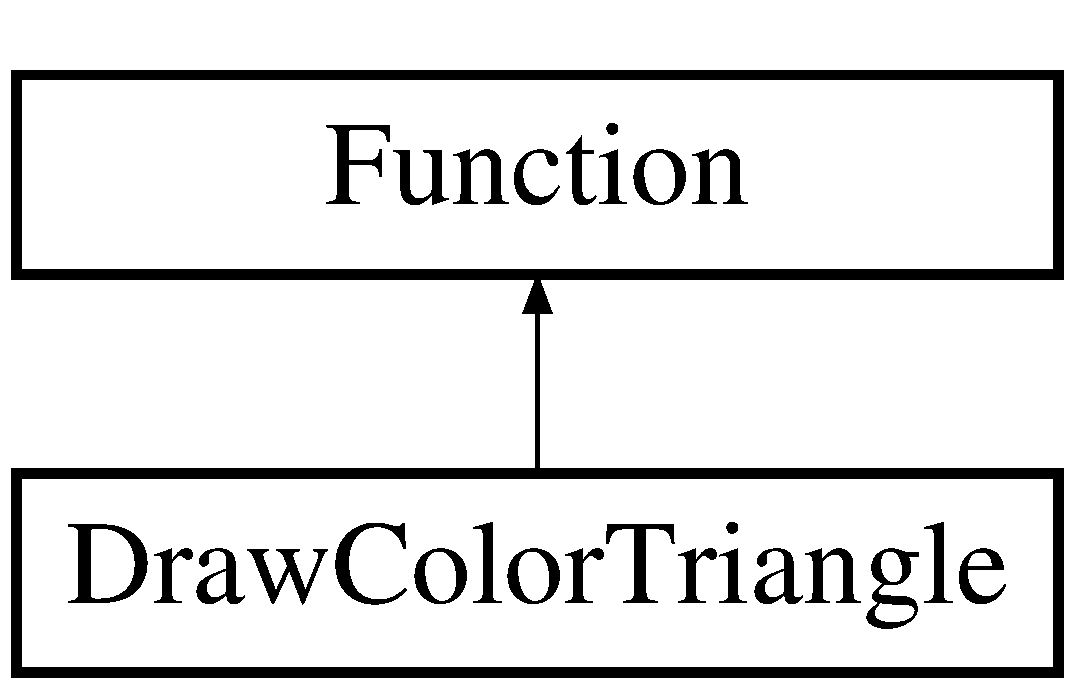
\includegraphics[height=2.000000cm]{class_draw_color_triangle}
\end{center}
\end{figure}
\subsection*{Public Member Functions}
\begin{DoxyCompactItemize}
\item 
\hypertarget{class_draw_color_triangle_a0bbb6e498405631981f2af8c30bed2a3}{{\bfseries Draw\-Color\-Triangle} (G\-P\-Config $\ast$conf)}\label{class_draw_color_triangle_a0bbb6e498405631981f2af8c30bed2a3}

\item 
\hypertarget{class_draw_color_triangle_a015d98a34270b2e0d50abc398cec39e3}{virtual void {\bfseries evaluate} (Return\-Data $\ast$out)}\label{class_draw_color_triangle_a015d98a34270b2e0d50abc398cec39e3}

\item 
\hypertarget{class_draw_color_triangle_a8854b0eedda24cb7e68088ea04fa3d31}{virtual Node $\ast$ {\bfseries copy} ()}\label{class_draw_color_triangle_a8854b0eedda24cb7e68088ea04fa3d31}

\end{DoxyCompactItemize}
\subsection*{Static Public Member Functions}
\begin{DoxyCompactItemize}
\item 
\hypertarget{class_draw_color_triangle_aafd3098c23fae0a80e8aae9297b9e490}{static Function $\ast$ {\bfseries generate} (const string \&name, G\-P\-Config $\ast$conf)}\label{class_draw_color_triangle_aafd3098c23fae0a80e8aae9297b9e490}

\end{DoxyCompactItemize}


The documentation for this class was generated from the following files\-:\begin{DoxyCompactItemize}
\item 
Draw\-Color\-Triangle.\-h\item 
Draw\-Color\-Triangle.\-cpp\end{DoxyCompactItemize}

\hypertarget{class_draw_gray_triangle}{\section{Draw\-Gray\-Triangle Class Reference}
\label{class_draw_gray_triangle}\index{Draw\-Gray\-Triangle@{Draw\-Gray\-Triangle}}
}
Inheritance diagram for Draw\-Gray\-Triangle\-:\begin{figure}[H]
\begin{center}
\leavevmode
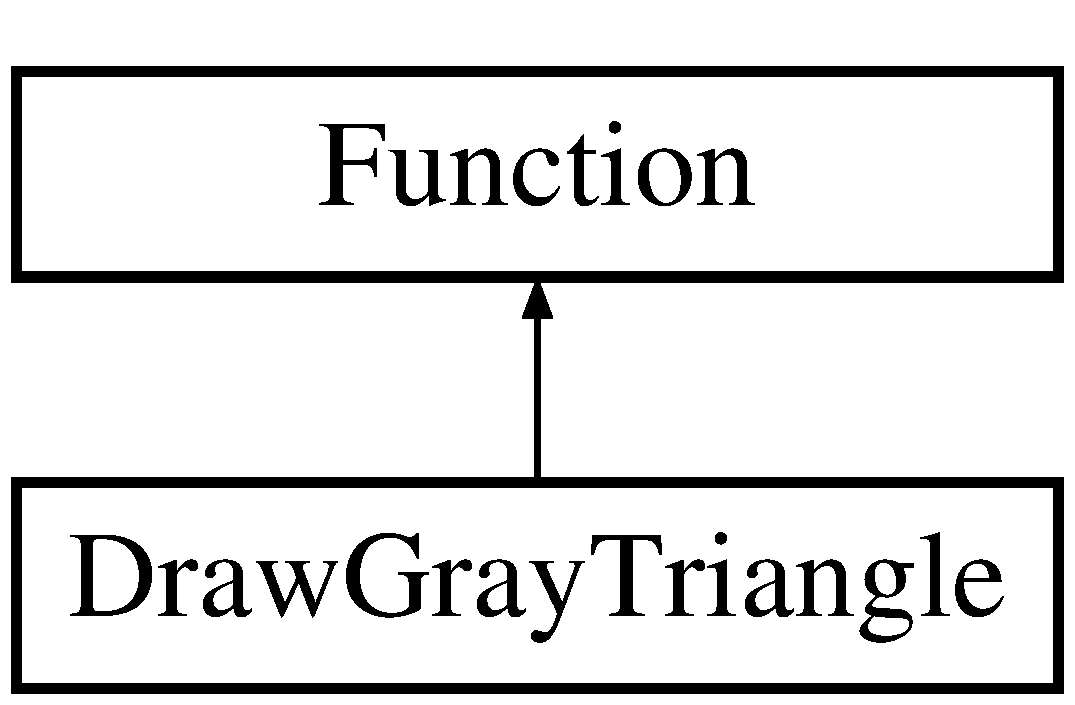
\includegraphics[height=2.000000cm]{class_draw_gray_triangle}
\end{center}
\end{figure}
\subsection*{Public Member Functions}
\begin{DoxyCompactItemize}
\item 
\hypertarget{class_draw_gray_triangle_a7a518e20ef8d09167ce78beb13c736cd}{{\bfseries Draw\-Gray\-Triangle} (G\-P\-Config $\ast$conf)}\label{class_draw_gray_triangle_a7a518e20ef8d09167ce78beb13c736cd}

\item 
\hypertarget{class_draw_gray_triangle_a17a78c3748736ef48dc8951b07361e68}{virtual void {\bfseries evaluate} (Return\-Data $\ast$out)}\label{class_draw_gray_triangle_a17a78c3748736ef48dc8951b07361e68}

\item 
\hypertarget{class_draw_gray_triangle_a085f4c505bbb6ff6e129649f29917276}{virtual Node $\ast$ {\bfseries copy} ()}\label{class_draw_gray_triangle_a085f4c505bbb6ff6e129649f29917276}

\end{DoxyCompactItemize}
\subsection*{Static Public Member Functions}
\begin{DoxyCompactItemize}
\item 
\hypertarget{class_draw_gray_triangle_ac9f2292e5d9b3709bb4f5fbb80a73e25}{static Function $\ast$ {\bfseries generate} (const string \&name, G\-P\-Config $\ast$conf)}\label{class_draw_gray_triangle_ac9f2292e5d9b3709bb4f5fbb80a73e25}

\end{DoxyCompactItemize}


The documentation for this class was generated from the following files\-:\begin{DoxyCompactItemize}
\item 
Draw\-Gray\-Triangle.\-h\item 
Draw\-Gray\-Triangle.\-cpp\end{DoxyCompactItemize}

\hypertarget{struct_h_s_v}{\section{H\-S\-V Struct Reference}
\label{struct_h_s_v}\index{H\-S\-V@{H\-S\-V}}
}
\subsection*{Public Attributes}
\begin{DoxyCompactItemize}
\item 
\hypertarget{struct_h_s_v_ab038be2f08af85438d55554c5580d79c}{int {\bfseries h}}\label{struct_h_s_v_ab038be2f08af85438d55554c5580d79c}

\item 
\hypertarget{struct_h_s_v_a9bb3f6690e6879d417c4488b81cf90ca}{int {\bfseries s}}\label{struct_h_s_v_a9bb3f6690e6879d417c4488b81cf90ca}

\item 
\hypertarget{struct_h_s_v_acf84a724f9e1478f30f1238ca487ad69}{int {\bfseries v}}\label{struct_h_s_v_acf84a724f9e1478f30f1238ca487ad69}

\end{DoxyCompactItemize}


The documentation for this struct was generated from the following file\-:\begin{DoxyCompactItemize}
\item 
Utility.\-h\end{DoxyCompactItemize}

\hypertarget{class_image_fitness}{\section{Image\-Fitness Class Reference}
\label{class_image_fitness}\index{Image\-Fitness@{Image\-Fitness}}
}
Inheritance diagram for Image\-Fitness\-:\begin{figure}[H]
\begin{center}
\leavevmode
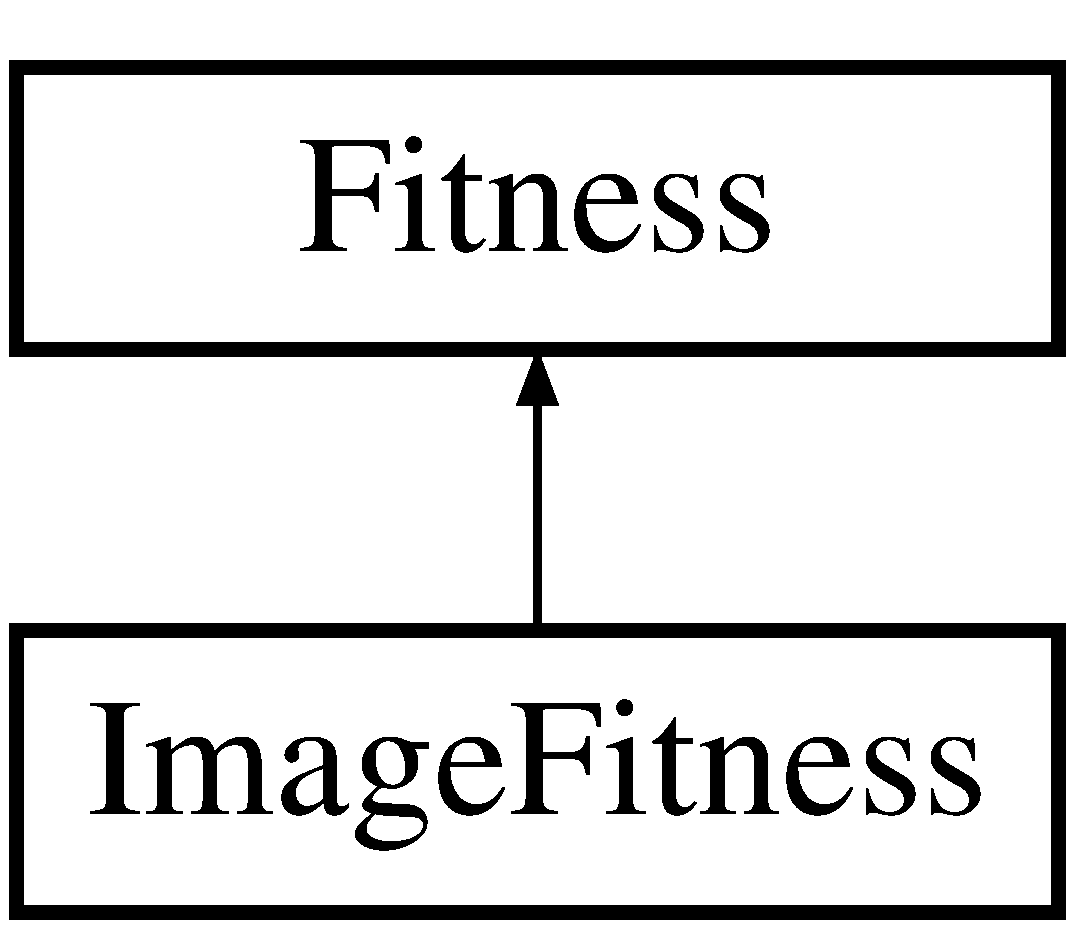
\includegraphics[height=2.000000cm]{class_image_fitness}
\end{center}
\end{figure}
\subsection*{Public Member Functions}
\begin{DoxyCompactItemize}
\item 
\hypertarget{class_image_fitness_abe7707371984af9215fcd812b51defef}{{\bfseries Image\-Fitness} (G\-P\-Config $\ast$conf)}\label{class_image_fitness_abe7707371984af9215fcd812b51defef}

\item 
\hypertarget{class_image_fitness_a87b7ded1718e3a5ddf41855e18c060d3}{virtual void {\bfseries init\-Fitness} ()}\label{class_image_fitness_a87b7ded1718e3a5ddf41855e18c060d3}

\item 
\hypertarget{class_image_fitness_ab7a09b58e0f1aa28eb54e92b1c7c1e39}{virtual void {\bfseries assign\-Fitness} (Genetic\-Program $\ast$pop\mbox{[}$\,$\mbox{]}, int pop\-Size)}\label{class_image_fitness_ab7a09b58e0f1aa28eb54e92b1c7c1e39}

\item 
\hypertarget{class_image_fitness_a20dad1b0e981f8d0e6f968982566b073}{virtual bool {\bfseries solution\-Found} (Genetic\-Program $\ast$pop\mbox{[}$\,$\mbox{]}, int pop\-Size)}\label{class_image_fitness_a20dad1b0e981f8d0e6f968982566b073}

\item 
\hypertarget{class_image_fitness_a8b981e2d67357f1316bce965da2cb511}{virtual bool {\bfseries is\-Better} (Genetic\-Program $\ast$gp1, Genetic\-Program $\ast$gp2)}\label{class_image_fitness_a8b981e2d67357f1316bce965da2cb511}

\item 
\hypertarget{class_image_fitness_ad140d00e2dd89edc72ebceadf8aaee00}{virtual bool {\bfseries is\-Worse} (Genetic\-Program $\ast$gp1, Genetic\-Program $\ast$gp2)}\label{class_image_fitness_ad140d00e2dd89edc72ebceadf8aaee00}

\item 
\hypertarget{class_image_fitness_a49732d7c1838113c37dae1bf102643e9}{virtual bool {\bfseries is\-Equal} (Genetic\-Program $\ast$gp1, Genetic\-Program $\ast$gp2)}\label{class_image_fitness_a49732d7c1838113c37dae1bf102643e9}

\item 
\hypertarget{class_image_fitness_a7906f6594096f7ebaf5e64bcfb56a657}{virtual double {\bfseries best} ()}\label{class_image_fitness_a7906f6594096f7ebaf5e64bcfb56a657}

\item 
\hypertarget{class_image_fitness_a58acec0b8d5e84da69221aab18308c47}{virtual double {\bfseries worst} ()}\label{class_image_fitness_a58acec0b8d5e84da69221aab18308c47}

\item 
\hypertarget{class_image_fitness_a3834397e9a1486dc37b2e4eb133bc84f}{void {\bfseries output\-Results} (Genetic\-Program $\ast$, char $\ast$, char $\ast$, double)}\label{class_image_fitness_a3834397e9a1486dc37b2e4eb133bc84f}

\end{DoxyCompactItemize}


The documentation for this class was generated from the following files\-:\begin{DoxyCompactItemize}
\item 
Image\-Fitness.\-h\item 
Image\-Fitness.\-cpp\end{DoxyCompactItemize}

\hypertarget{class_mask_maker}{\section{Mask\-Maker Class Reference}
\label{class_mask_maker}\index{Mask\-Maker@{Mask\-Maker}}
}
\subsection*{Public Member Functions}
\begin{DoxyCompactItemize}
\item 
\hypertarget{class_mask_maker_a94e5e9132a4dd3e4e1d8d1cdc8e0fcd2}{{\bfseries Mask\-Maker} (const char $\ast$source\-File, const char $\ast$output\-File, unsigned T, unsigned N)}\label{class_mask_maker_a94e5e9132a4dd3e4e1d8d1cdc8e0fcd2}

\item 
\hypertarget{class_mask_maker_a0fe6264b064fa722664f2eefb73af9e1}{void {\bfseries make\-Default\-Mask} ()}\label{class_mask_maker_a0fe6264b064fa722664f2eefb73af9e1}

\end{DoxyCompactItemize}


The documentation for this class was generated from the following files\-:\begin{DoxyCompactItemize}
\item 
Mask\-Maker.\-h\item 
Mask\-Maker.\-cpp\end{DoxyCompactItemize}

\hypertarget{class_palette}{\section{Palette Class Reference}
\label{class_palette}\index{Palette@{Palette}}
}
\subsection*{Public Member Functions}
\begin{DoxyCompactItemize}
\item 
\hypertarget{class_palette_a9e7d1cfc83132e54f881c95acf0cb0d9}{{\bfseries Palette} (\hyperlink{class_target}{Target} $\ast$target)}\label{class_palette_a9e7d1cfc83132e54f881c95acf0cb0d9}

\item 
\hypertarget{class_palette_ab861218bb6b4b64f24c774deaf26cada}{{\bfseries Palette} (const char $\ast$)}\label{class_palette_ab861218bb6b4b64f24c774deaf26cada}

\item 
\hypertarget{class_palette_abec7160109e458ab445ba1eaf752ab85}{\hyperlink{struct_r_g_b}{R\-G\-B} {\bfseries get\-Random\-R\-G\-B} (float f)}\label{class_palette_abec7160109e458ab445ba1eaf752ab85}

\item 
\hypertarget{class_palette_a11248e33e13b761d483f251ec21d9d11}{\hyperlink{struct_h_s_v}{H\-S\-V} {\bfseries get\-Random\-H\-S\-V} (float f)}\label{class_palette_a11248e33e13b761d483f251ec21d9d11}

\end{DoxyCompactItemize}


The documentation for this class was generated from the following files\-:\begin{DoxyCompactItemize}
\item 
Palette.\-h\item 
Palette.\-cpp\end{DoxyCompactItemize}

\hypertarget{class_pixel}{\section{Pixel Class Reference}
\label{class_pixel}\index{Pixel@{Pixel}}
}
\subsection*{Public Member Functions}
\begin{DoxyCompactItemize}
\item 
\hypertarget{class_pixel_afe2eb7843df8e519d6abc8b9d4df9688}{{\bfseries Pixel} (\hyperlink{struct_r_g_b}{R\-G\-B})}\label{class_pixel_afe2eb7843df8e519d6abc8b9d4df9688}

\item 
\hypertarget{class_pixel_a5099935f8ed4a93fc04fe94e9897b721}{{\bfseries Pixel} (\hyperlink{struct_h_s_v}{H\-S\-V})}\label{class_pixel_a5099935f8ed4a93fc04fe94e9897b721}

\item 
\hypertarget{class_pixel_a123fe9b4701578656ce46429001ea301}{\hyperlink{struct_r_g_b}{R\-G\-B} {\bfseries get\-R\-G\-B} ()}\label{class_pixel_a123fe9b4701578656ce46429001ea301}

\item 
\hypertarget{class_pixel_adb6c4a94e33ac4029577ce7304ee43dc}{\hyperlink{struct_h_s_v}{H\-S\-V} {\bfseries get\-H\-S\-V} ()}\label{class_pixel_adb6c4a94e33ac4029577ce7304ee43dc}

\item 
\hypertarget{class_pixel_a6e0eb6c9581fbde8e13fd771ff88ada6}{color\-\_\-t {\bfseries get\-R} ()}\label{class_pixel_a6e0eb6c9581fbde8e13fd771ff88ada6}

\item 
\hypertarget{class_pixel_a69bf3cfda8d9543593764c9f2692ba26}{color\-\_\-t {\bfseries get\-G} ()}\label{class_pixel_a69bf3cfda8d9543593764c9f2692ba26}

\item 
\hypertarget{class_pixel_a4249cdc22eb5d95d89928f9f1640849e}{color\-\_\-t {\bfseries get\-B} ()}\label{class_pixel_a4249cdc22eb5d95d89928f9f1640849e}

\item 
\hypertarget{class_pixel_a2b9de1d5e1cf04b38a1cbc5a298543d6}{int {\bfseries get\-H} () const }\label{class_pixel_a2b9de1d5e1cf04b38a1cbc5a298543d6}

\item 
\hypertarget{class_pixel_aa3933520159a789f3a7b819e6d8e4bc6}{int {\bfseries get\-S} () const }\label{class_pixel_aa3933520159a789f3a7b819e6d8e4bc6}

\item 
\hypertarget{class_pixel_a921f6b0a83075c52491280eeec29e38b}{int {\bfseries get\-V} () const }\label{class_pixel_a921f6b0a83075c52491280eeec29e38b}

\item 
\hypertarget{class_pixel_a3a632ce38ad1a93a65406114f08cd628}{void {\bfseries set\-Color} (\hyperlink{struct_r_g_b}{R\-G\-B})}\label{class_pixel_a3a632ce38ad1a93a65406114f08cd628}

\item 
\hypertarget{class_pixel_a1d004a491b2c5ee95880a70d7cf21b86}{void {\bfseries set\-Color} (\hyperlink{struct_h_s_v}{H\-S\-V})}\label{class_pixel_a1d004a491b2c5ee95880a70d7cf21b86}

\item 
\hypertarget{class_pixel_a7669a7187a0d2a009de71c77871b58de}{void {\bfseries set\-R} (color\-\_\-t channel)}\label{class_pixel_a7669a7187a0d2a009de71c77871b58de}

\item 
\hypertarget{class_pixel_a3d4e74403f26074ba90a426d993088a9}{void {\bfseries set\-G} (color\-\_\-t channel)}\label{class_pixel_a3d4e74403f26074ba90a426d993088a9}

\item 
\hypertarget{class_pixel_ae1af48d6d61212522a678e3dc4daa22e}{void {\bfseries set\-B} (color\-\_\-t channel)}\label{class_pixel_ae1af48d6d61212522a678e3dc4daa22e}

\item 
\hypertarget{class_pixel_a9235a7497036c9066feeb8d019791bdc}{void {\bfseries set\-H} (int channel)}\label{class_pixel_a9235a7497036c9066feeb8d019791bdc}

\item 
\hypertarget{class_pixel_a0414e865cfc3a1e451f7a80cd7f165b8}{void {\bfseries set\-S} (int channel)}\label{class_pixel_a0414e865cfc3a1e451f7a80cd7f165b8}

\item 
\hypertarget{class_pixel_aa86fd55d3fd189062f94f3e557d3b988}{void {\bfseries set\-V} (int channel)}\label{class_pixel_aa86fd55d3fd189062f94f3e557d3b988}

\item 
\hypertarget{class_pixel_af81a1dc95e90fe9bf836c0e3b27cdbba}{bool {\bfseries operator$<$} (const \hyperlink{class_pixel}{Pixel} \&)}\label{class_pixel_af81a1dc95e90fe9bf836c0e3b27cdbba}

\item 
\hypertarget{class_pixel_a0b56df19ddd3e7b7c53107047ff9083b}{bool {\bfseries operator=} (const \hyperlink{class_pixel}{Pixel} \&)}\label{class_pixel_a0b56df19ddd3e7b7c53107047ff9083b}

\item 
\hypertarget{class_pixel_abded9446d55db7ec7eff0beb52d5c5a4}{void {\bfseries to\-String} ()}\label{class_pixel_abded9446d55db7ec7eff0beb52d5c5a4}

\end{DoxyCompactItemize}


The documentation for this class was generated from the following files\-:\begin{DoxyCompactItemize}
\item 
Pixel.\-h\item 
Pixel.\-cpp\end{DoxyCompactItemize}

\hypertarget{class_prog2}{\section{Prog2 Class Reference}
\label{class_prog2}\index{Prog2@{Prog2}}
}
Inheritance diagram for Prog2\-:\begin{figure}[H]
\begin{center}
\leavevmode
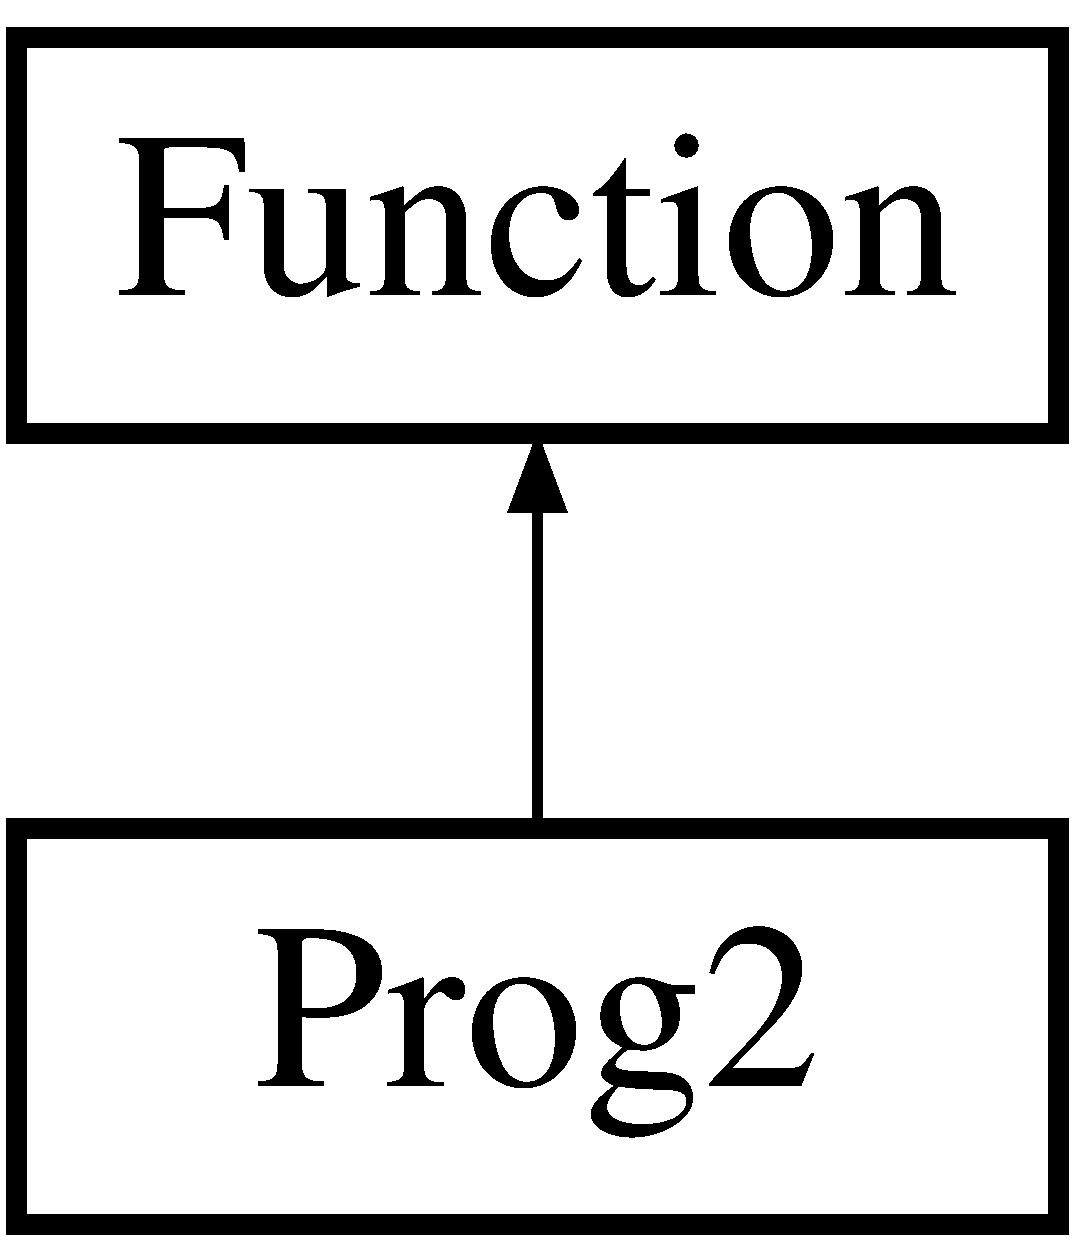
\includegraphics[height=2.000000cm]{class_prog2}
\end{center}
\end{figure}
\subsection*{Public Member Functions}
\begin{DoxyCompactItemize}
\item 
\hypertarget{class_prog2_a484a9c7ee3c73a01e04a6c40a724ba70}{{\bfseries Prog2} (G\-P\-Config $\ast$conf)}\label{class_prog2_a484a9c7ee3c73a01e04a6c40a724ba70}

\item 
\hypertarget{class_prog2_a119d9652b5ad96835e3aa49feeecfbda}{virtual void {\bfseries evaluate} (Return\-Data $\ast$out)}\label{class_prog2_a119d9652b5ad96835e3aa49feeecfbda}

\item 
\hypertarget{class_prog2_ab08249153b686963d3991d25d78f6827}{virtual Node $\ast$ {\bfseries copy} ()}\label{class_prog2_ab08249153b686963d3991d25d78f6827}

\end{DoxyCompactItemize}
\subsection*{Static Public Member Functions}
\begin{DoxyCompactItemize}
\item 
\hypertarget{class_prog2_a6c0efb0ed015721372c384c2dab8cf2e}{static Function $\ast$ {\bfseries generate} (const string \&name, G\-P\-Config $\ast$conf)}\label{class_prog2_a6c0efb0ed015721372c384c2dab8cf2e}

\end{DoxyCompactItemize}


The documentation for this class was generated from the following files\-:\begin{DoxyCompactItemize}
\item 
Prog2.\-h\item 
Prog2.\-cpp\end{DoxyCompactItemize}

\hypertarget{class_prog3}{\section{Prog3 Class Reference}
\label{class_prog3}\index{Prog3@{Prog3}}
}
Inheritance diagram for Prog3\-:\begin{figure}[H]
\begin{center}
\leavevmode
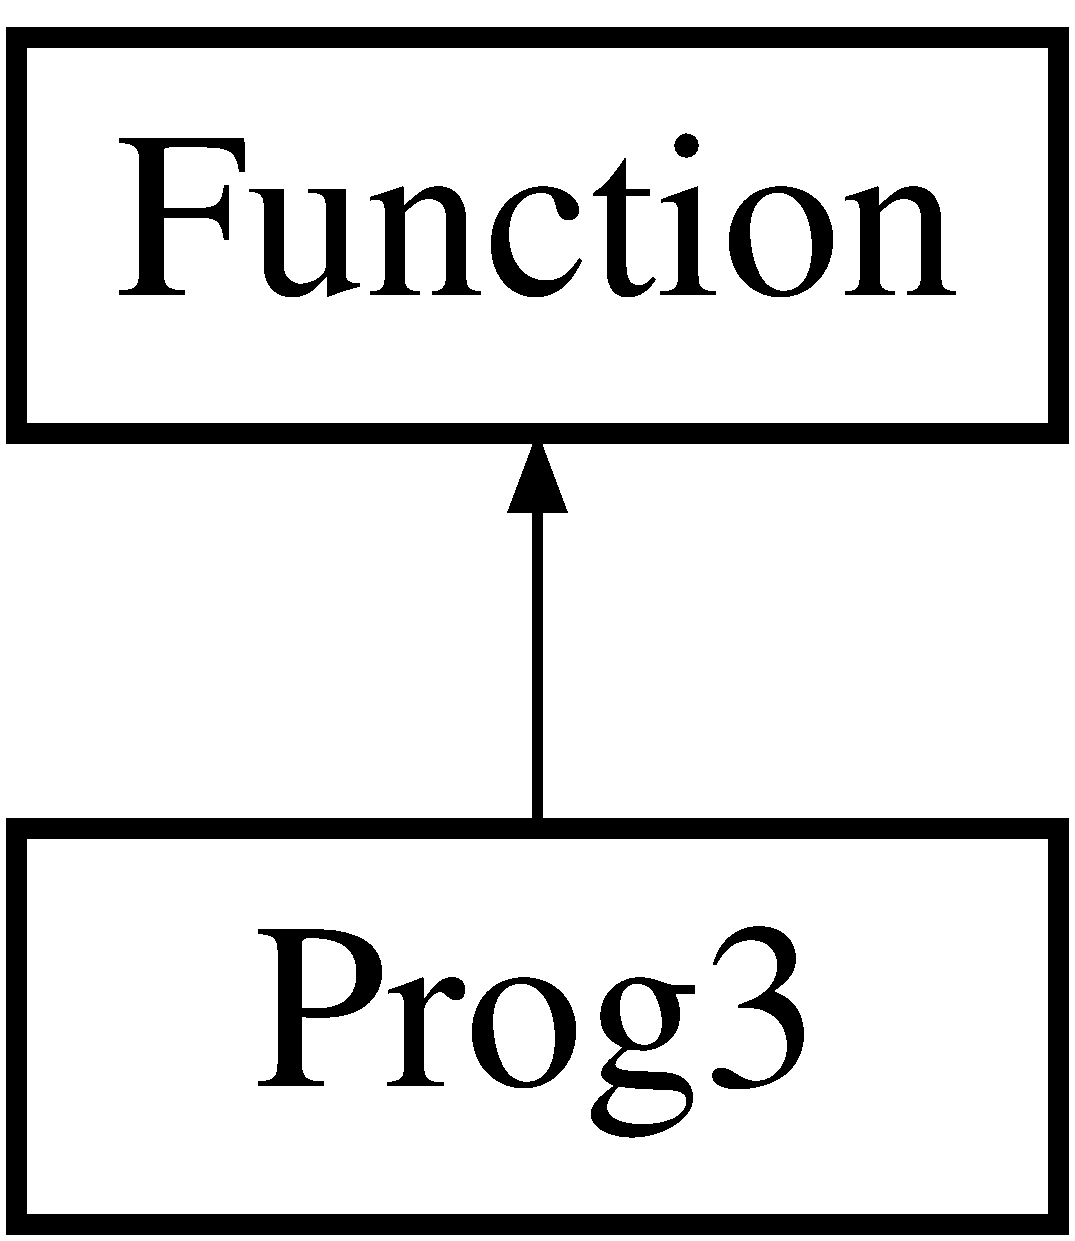
\includegraphics[height=2.000000cm]{class_prog3}
\end{center}
\end{figure}
\subsection*{Public Member Functions}
\begin{DoxyCompactItemize}
\item 
\hypertarget{class_prog3_a97abd230e67701241ff9b55211813175}{{\bfseries Prog3} (G\-P\-Config $\ast$conf)}\label{class_prog3_a97abd230e67701241ff9b55211813175}

\item 
\hypertarget{class_prog3_a03860caf456da8eca8a9e2e324d7df05}{virtual void {\bfseries evaluate} (Return\-Data $\ast$out)}\label{class_prog3_a03860caf456da8eca8a9e2e324d7df05}

\item 
\hypertarget{class_prog3_a398d905914e1a6d7bb81ad97f97e9fa1}{virtual Node $\ast$ {\bfseries copy} ()}\label{class_prog3_a398d905914e1a6d7bb81ad97f97e9fa1}

\end{DoxyCompactItemize}
\subsection*{Static Public Member Functions}
\begin{DoxyCompactItemize}
\item 
\hypertarget{class_prog3_a3632b942186a76c3eac8b2c97b964d62}{static Function $\ast$ {\bfseries generate} (const string \&name, G\-P\-Config $\ast$conf)}\label{class_prog3_a3632b942186a76c3eac8b2c97b964d62}

\end{DoxyCompactItemize}


The documentation for this class was generated from the following files\-:\begin{DoxyCompactItemize}
\item 
Prog3.\-h\item 
Prog3.\-cpp\end{DoxyCompactItemize}

\hypertarget{class_prog4}{\section{Prog4 Class Reference}
\label{class_prog4}\index{Prog4@{Prog4}}
}
Inheritance diagram for Prog4\-:\begin{figure}[H]
\begin{center}
\leavevmode
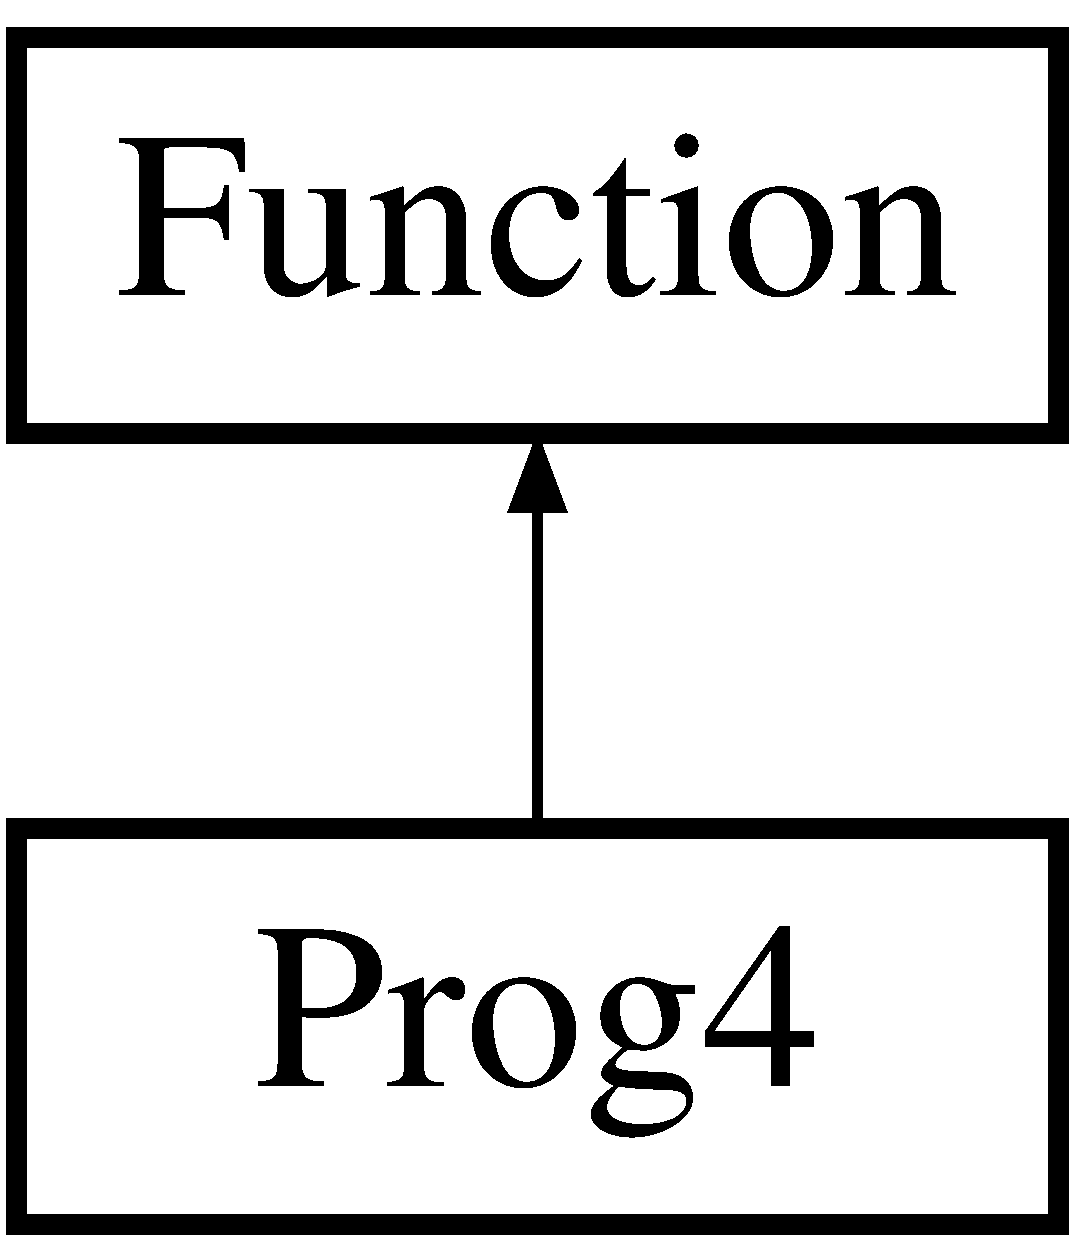
\includegraphics[height=2.000000cm]{class_prog4}
\end{center}
\end{figure}
\subsection*{Public Member Functions}
\begin{DoxyCompactItemize}
\item 
\hypertarget{class_prog4_a5e86ff04b5e8652f917f2a838fa6b0aa}{{\bfseries Prog4} (G\-P\-Config $\ast$conf)}\label{class_prog4_a5e86ff04b5e8652f917f2a838fa6b0aa}

\item 
\hypertarget{class_prog4_a2bd6ea497e7e6d4ab5c109dd37ced620}{virtual void {\bfseries evaluate} (Return\-Data $\ast$out)}\label{class_prog4_a2bd6ea497e7e6d4ab5c109dd37ced620}

\item 
\hypertarget{class_prog4_a855801b596cb17fe45c8fde5c701ea08}{virtual Node $\ast$ {\bfseries copy} ()}\label{class_prog4_a855801b596cb17fe45c8fde5c701ea08}

\end{DoxyCompactItemize}
\subsection*{Static Public Member Functions}
\begin{DoxyCompactItemize}
\item 
\hypertarget{class_prog4_a4a828b4aadd8faac2f642ab2bdd45d58}{static Function $\ast$ {\bfseries generate} (const string \&name, G\-P\-Config $\ast$conf)}\label{class_prog4_a4a828b4aadd8faac2f642ab2bdd45d58}

\end{DoxyCompactItemize}


The documentation for this class was generated from the following files\-:\begin{DoxyCompactItemize}
\item 
Prog4.\-h\item 
Prog4.\-cpp\end{DoxyCompactItemize}

\hypertarget{class_ralph}{\section{Ralph Class Reference}
\label{class_ralph}\index{Ralph@{Ralph}}
}
\subsection*{Public Member Functions}
\begin{DoxyCompactItemize}
\item 
\hypertarget{class_ralph_ab269d8a3ad97335078fe1dbe2c125ff6}{double {\bfseries compute\-R\-G\-B\-Image} (\hyperlink{struct_r_g_b}{R\-G\-B} $\ast$image, int width, int height)}\label{class_ralph_ab269d8a3ad97335078fe1dbe2c125ff6}

\item 
\hypertarget{class_ralph_a139bcc99790667b998a48719b20e9b2a}{double {\bfseries compute\-H\-S\-V\-Image} (\hyperlink{struct_h_s_v}{H\-S\-V} $\ast$image, int width, int height)}\label{class_ralph_a139bcc99790667b998a48719b20e9b2a}

\end{DoxyCompactItemize}


The documentation for this class was generated from the following files\-:\begin{DoxyCompactItemize}
\item 
Ralph.\-h\item 
Ralph.\-cpp\end{DoxyCompactItemize}

\hypertarget{class_rand_float}{\section{Rand\-Float Class Reference}
\label{class_rand_float}\index{Rand\-Float@{Rand\-Float}}
}
Inheritance diagram for Rand\-Float\-:\begin{figure}[H]
\begin{center}
\leavevmode
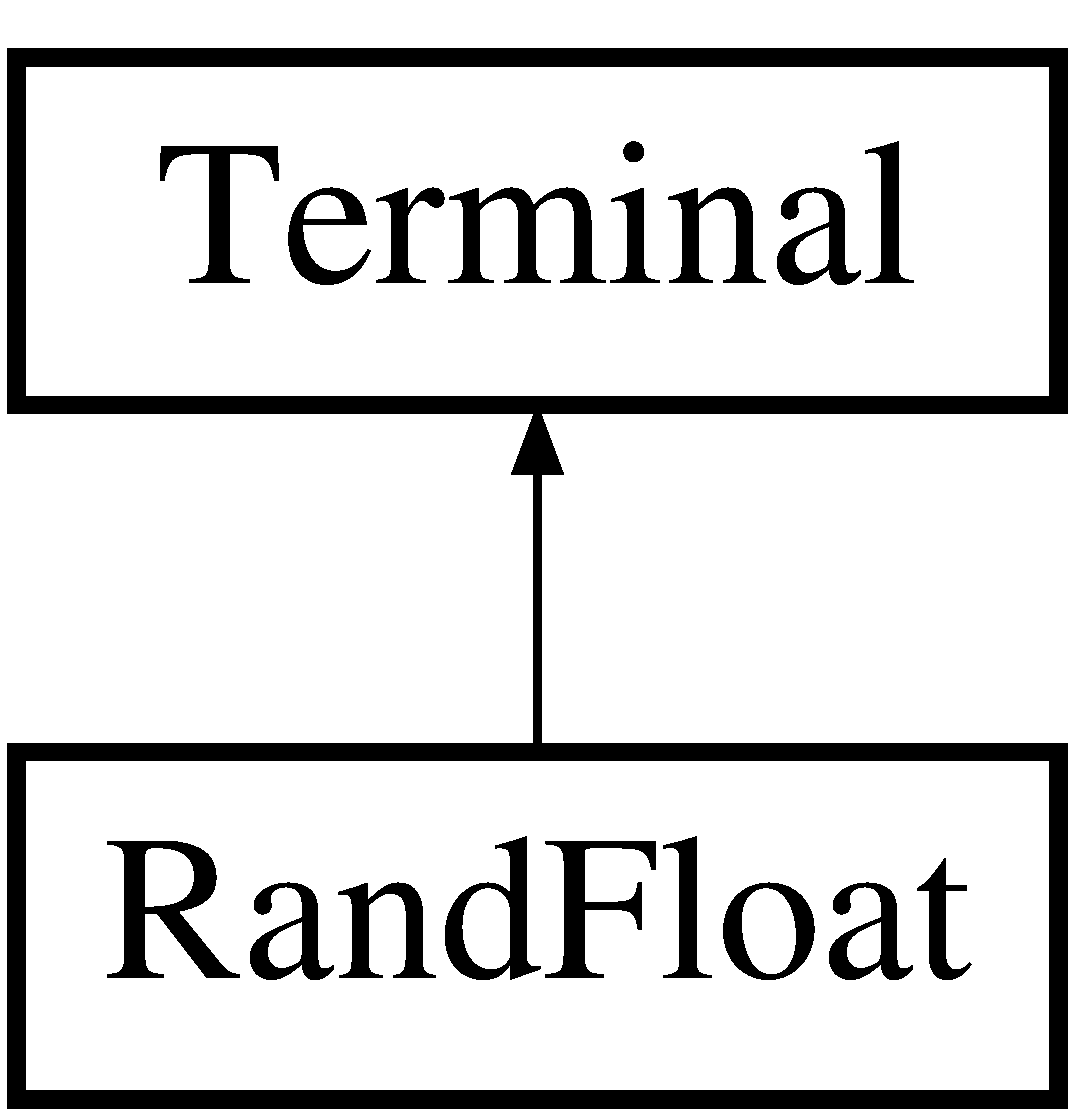
\includegraphics[height=2.000000cm]{class_rand_float}
\end{center}
\end{figure}
\subsection*{Public Member Functions}
\begin{DoxyCompactItemize}
\item 
\hypertarget{class_rand_float_a5e94dcef866954df6b152fb8d2a5e5b7}{{\bfseries Rand\-Float} (G\-P\-Config $\ast$conf)}\label{class_rand_float_a5e94dcef866954df6b152fb8d2a5e5b7}

\item 
\hypertarget{class_rand_float_abb7becde66cc9884bfa23dc8b73b40be}{{\bfseries Rand\-Float} (float init\-Value, G\-P\-Config $\ast$conf)}\label{class_rand_float_abb7becde66cc9884bfa23dc8b73b40be}

\item 
\hypertarget{class_rand_float_a6207a53aae9ddde61b4df865a12a5761}{virtual void {\bfseries evaluate} (Return\-Data $\ast$out)}\label{class_rand_float_a6207a53aae9ddde61b4df865a12a5761}

\item 
\hypertarget{class_rand_float_a1080521794c25b5ab881dab1d829bb80}{virtual void {\bfseries print} (string \&s)}\label{class_rand_float_a1080521794c25b5ab881dab1d829bb80}

\item 
\hypertarget{class_rand_float_a1c86fd91edd14ffef050a9b610cfec17}{virtual Node $\ast$ {\bfseries copy} ()}\label{class_rand_float_a1c86fd91edd14ffef050a9b610cfec17}

\end{DoxyCompactItemize}
\subsection*{Static Public Member Functions}
\begin{DoxyCompactItemize}
\item 
\hypertarget{class_rand_float_a8ab1360b98f5c6cdeec81de6910b9004}{static Terminal $\ast$ {\bfseries generate} (const string \&name, G\-P\-Config $\ast$conf)}\label{class_rand_float_a8ab1360b98f5c6cdeec81de6910b9004}

\end{DoxyCompactItemize}


The documentation for this class was generated from the following files\-:\begin{DoxyCompactItemize}
\item 
Rand\-Float.\-h\item 
Rand\-Float.\-cpp\end{DoxyCompactItemize}

\hypertarget{class_return_float}{\section{Return\-Float Class Reference}
\label{class_return_float}\index{Return\-Float@{Return\-Float}}
}
Inheritance diagram for Return\-Float\-:\begin{figure}[H]
\begin{center}
\leavevmode
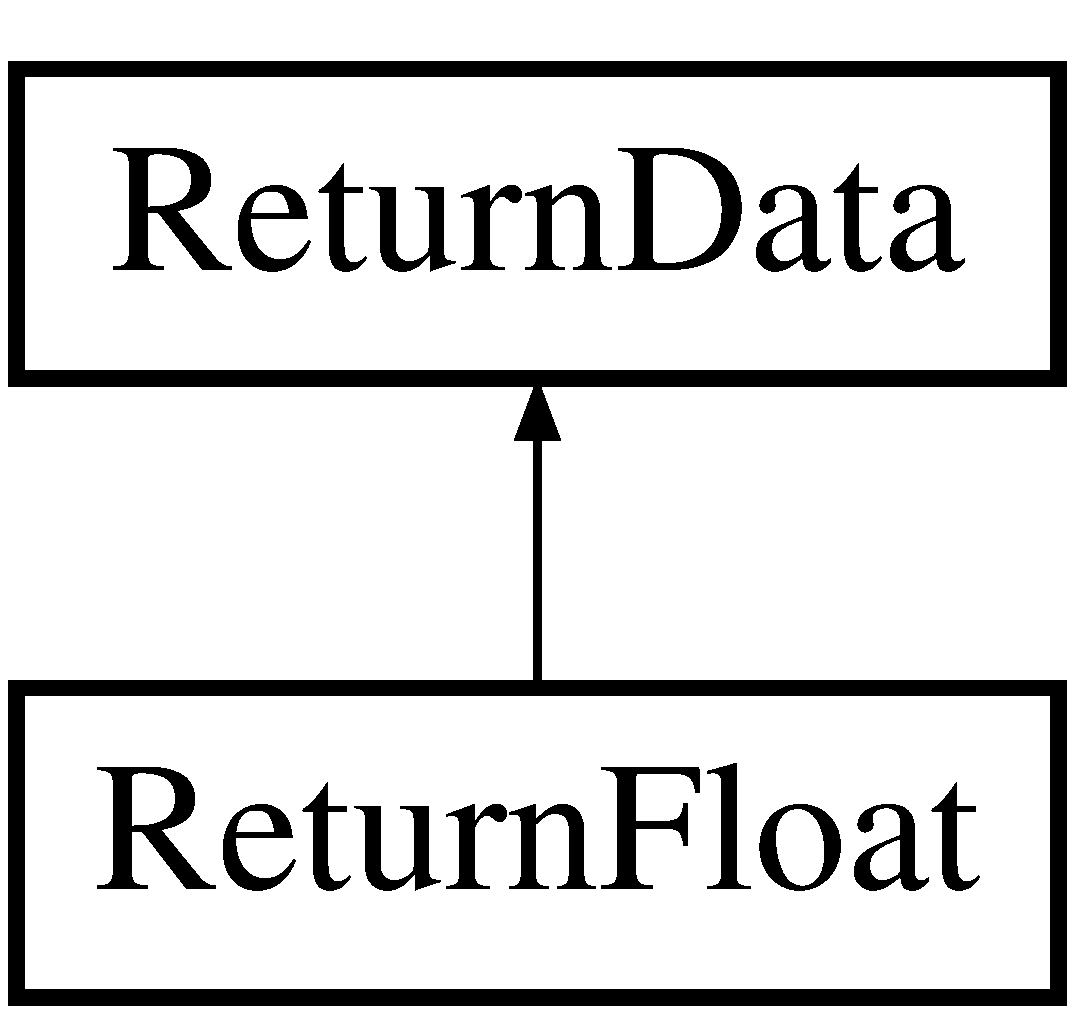
\includegraphics[height=2.000000cm]{class_return_float}
\end{center}
\end{figure}
\subsection*{Public Member Functions}
\begin{DoxyCompactItemize}
\item 
\hypertarget{class_return_float_a3d8aea3ea6e416098554dfd157cb60eb}{void {\bfseries set\-Data} (float num)}\label{class_return_float_a3d8aea3ea6e416098554dfd157cb60eb}

\item 
\hypertarget{class_return_float_afa93a257baac8ee3d9812851bf44cbb8}{float {\bfseries get\-Data} () const }\label{class_return_float_afa93a257baac8ee3d9812851bf44cbb8}

\end{DoxyCompactItemize}
\subsection*{Static Public Attributes}
\begin{DoxyCompactItemize}
\item 
\hypertarget{class_return_float_aba14d134e5986c2c8e706a6a6107e867}{static const int {\bfseries T\-Y\-P\-E\-N\-U\-M} = 2}\label{class_return_float_aba14d134e5986c2c8e706a6a6107e867}

\end{DoxyCompactItemize}


The documentation for this class was generated from the following files\-:\begin{DoxyCompactItemize}
\item 
Return\-Float.\-h\item 
Return\-Float.\-cpp\end{DoxyCompactItemize}

\hypertarget{class_return_func}{\section{Return\-Func Class Reference}
\label{class_return_func}\index{Return\-Func@{Return\-Func}}
}
Inheritance diagram for Return\-Func\-:\begin{figure}[H]
\begin{center}
\leavevmode
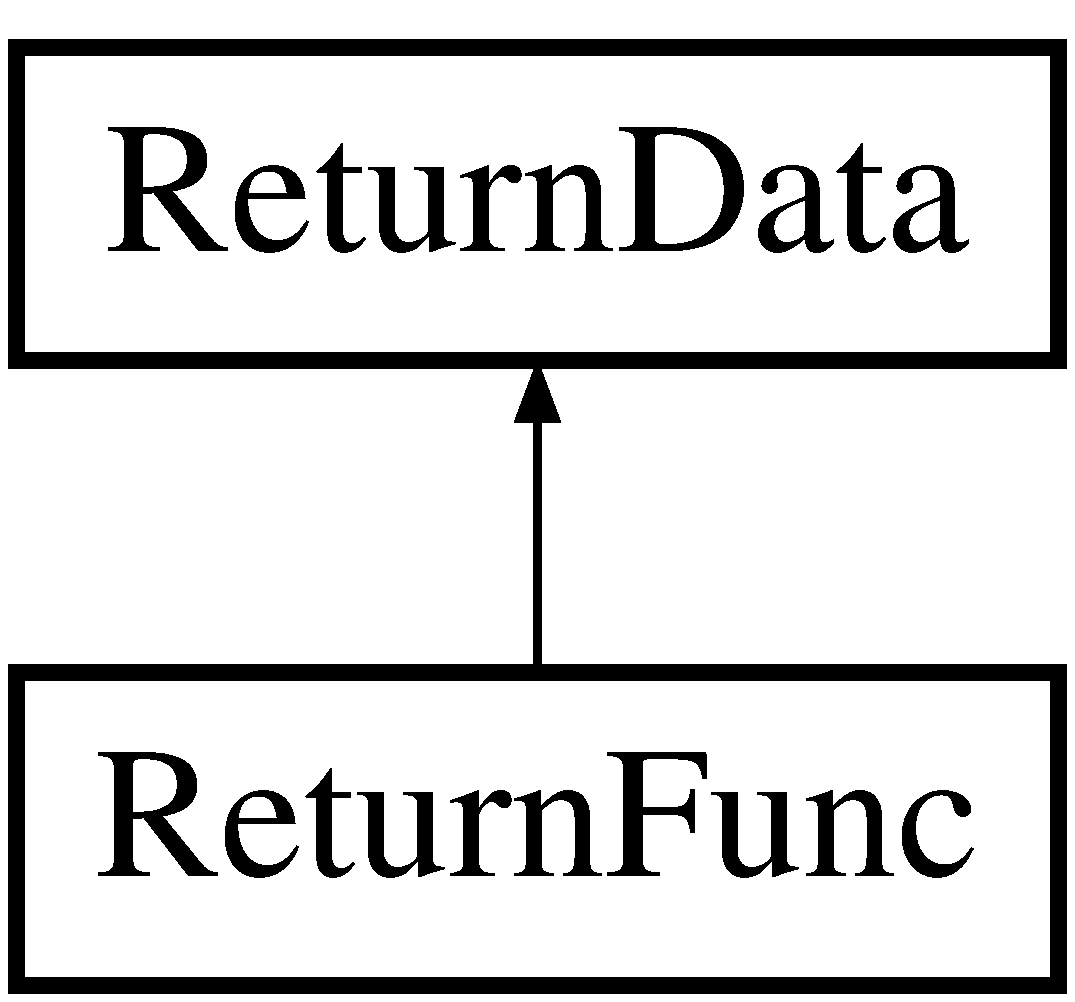
\includegraphics[height=2.000000cm]{class_return_func}
\end{center}
\end{figure}
\subsection*{Public Member Functions}
\begin{DoxyCompactItemize}
\item 
\hypertarget{class_return_func_acece0b291362fedc2ffb85260d7265ef}{void {\bfseries set\-Data} (float num)}\label{class_return_func_acece0b291362fedc2ffb85260d7265ef}

\item 
\hypertarget{class_return_func_a923b08b85b05c1884b2382b27b62a9c7}{float {\bfseries get\-Data} () const }\label{class_return_func_a923b08b85b05c1884b2382b27b62a9c7}

\end{DoxyCompactItemize}
\subsection*{Static Public Attributes}
\begin{DoxyCompactItemize}
\item 
\hypertarget{class_return_func_af1d2ac69deb830ac09527db1a0938a32}{static const int {\bfseries T\-Y\-P\-E\-N\-U\-M} = 1}\label{class_return_func_af1d2ac69deb830ac09527db1a0938a32}

\end{DoxyCompactItemize}


The documentation for this class was generated from the following files\-:\begin{DoxyCompactItemize}
\item 
Return\-Func.\-h\item 
Return\-Func.\-cpp\end{DoxyCompactItemize}

\hypertarget{class_return_root}{\section{Return\-Root Class Reference}
\label{class_return_root}\index{Return\-Root@{Return\-Root}}
}
Inheritance diagram for Return\-Root\-:\begin{figure}[H]
\begin{center}
\leavevmode
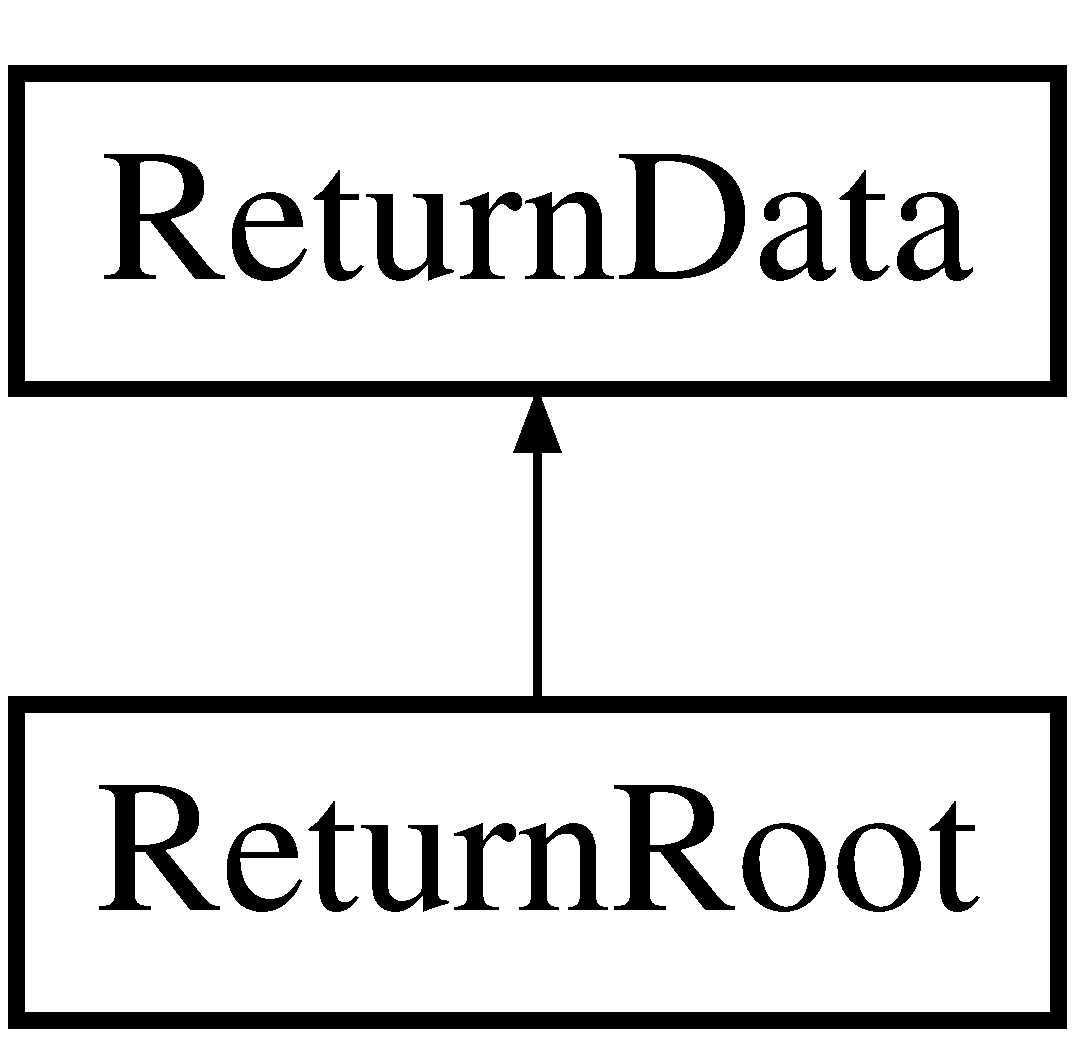
\includegraphics[height=2.000000cm]{class_return_root}
\end{center}
\end{figure}
\subsection*{Public Member Functions}
\begin{DoxyCompactItemize}
\item 
\hypertarget{class_return_root_aee0234acc3e276cee21e7acd2e51f4b9}{void {\bfseries set\-Data} (float num)}\label{class_return_root_aee0234acc3e276cee21e7acd2e51f4b9}

\item 
\hypertarget{class_return_root_a3514cad08617cef13e9a2671196ca0b9}{float {\bfseries get\-Data} () const }\label{class_return_root_a3514cad08617cef13e9a2671196ca0b9}

\end{DoxyCompactItemize}
\subsection*{Static Public Attributes}
\begin{DoxyCompactItemize}
\item 
\hypertarget{class_return_root_af8b144313269a7cc5475dcc8c3b69da4}{static const int {\bfseries T\-Y\-P\-E\-N\-U\-M} = 0}\label{class_return_root_af8b144313269a7cc5475dcc8c3b69da4}

\end{DoxyCompactItemize}


The documentation for this class was generated from the following files\-:\begin{DoxyCompactItemize}
\item 
Return\-Root.\-h\item 
Return\-Root.\-cpp\end{DoxyCompactItemize}

\hypertarget{struct_r_g_b}{\section{R\-G\-B Struct Reference}
\label{struct_r_g_b}\index{R\-G\-B@{R\-G\-B}}
}
\subsection*{Public Attributes}
\begin{DoxyCompactItemize}
\item 
\hypertarget{struct_r_g_b_a8ea970fcd312802ef238733b1c9ed63d}{unsigned char {\bfseries r}}\label{struct_r_g_b_a8ea970fcd312802ef238733b1c9ed63d}

\item 
\hypertarget{struct_r_g_b_a3595e9a2ed44c815153aff4e84e2d97c}{unsigned char {\bfseries g}}\label{struct_r_g_b_a3595e9a2ed44c815153aff4e84e2d97c}

\item 
\hypertarget{struct_r_g_b_ab2a3ac761d61594e2c51d65347a74017}{unsigned char {\bfseries b}}\label{struct_r_g_b_ab2a3ac761d61594e2c51d65347a74017}

\end{DoxyCompactItemize}


The documentation for this struct was generated from the following file\-:\begin{DoxyCompactItemize}
\item 
Utility.\-h\end{DoxyCompactItemize}

\hypertarget{class_shroud_canvas}{\section{Shroud\-Canvas Class Reference}
\label{class_shroud_canvas}\index{Shroud\-Canvas@{Shroud\-Canvas}}
}
Inheritance diagram for Shroud\-Canvas\-:\begin{figure}[H]
\begin{center}
\leavevmode
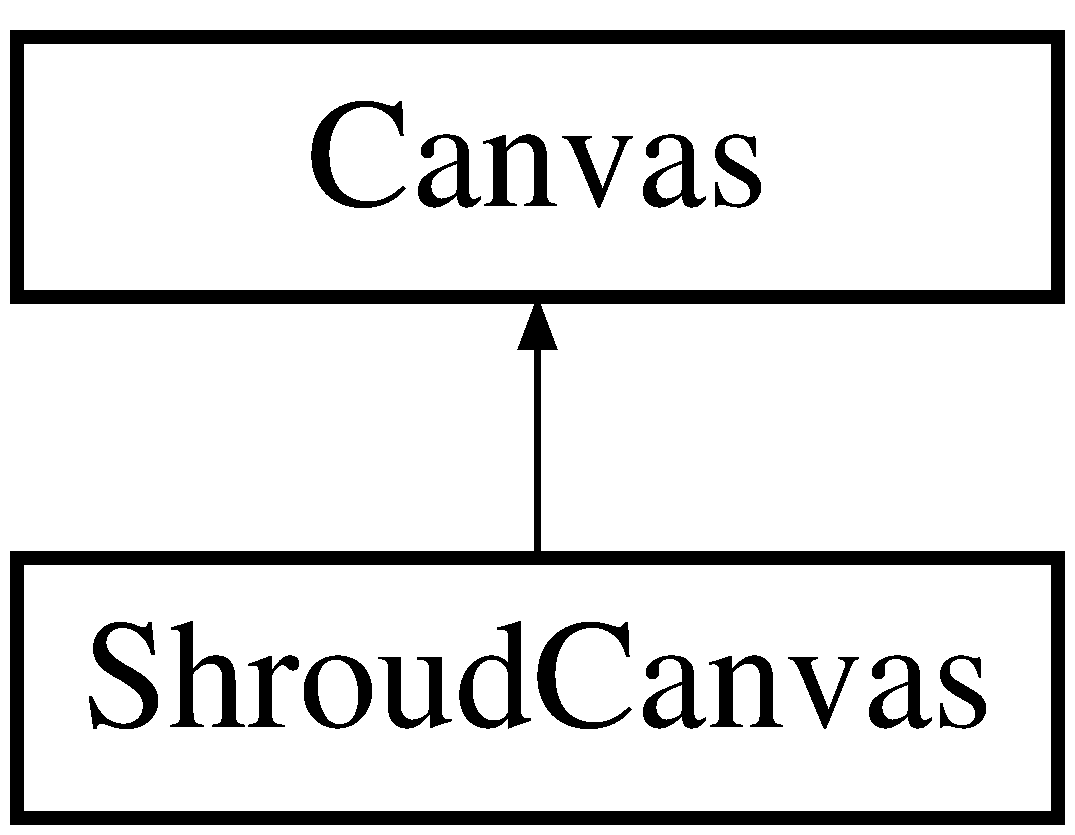
\includegraphics[height=2.000000cm]{class_shroud_canvas}
\end{center}
\end{figure}
\subsection*{Public Member Functions}
\begin{DoxyCompactItemize}
\item 
\hypertarget{class_shroud_canvas_a7723ea991bc0b77b24c9480be58c0728}{{\bfseries Shroud\-Canvas} (\hyperlink{class_target}{Target} $\ast$t, color\-\_\-t bg\-\_\-\-Red, color\-\_\-t bg\-\_\-\-Green, color\-\_\-t bg\-\_\-\-Blue, \hyperlink{class_best_canvas}{Best\-Canvas} $\ast$bc, \hyperlink{class_config_reader}{Config\-Reader} $\ast$reader)}\label{class_shroud_canvas_a7723ea991bc0b77b24c9480be58c0728}

\item 
\hypertarget{class_shroud_canvas_a0b43672515fb0e4119e907fc97682d32}{void {\bfseries fast\-Colour\-Technique3} (\hyperlink{struct_r_g_b}{R\-G\-B} target\-Pixel, \hyperlink{struct_r_g_b}{R\-G\-B} canvas\-Pixel, \hyperlink{struct_r_g_b}{R\-G\-B} line\-Color, \hyperlink{struct_coord}{Coord} c)}\label{class_shroud_canvas_a0b43672515fb0e4119e907fc97682d32}

\item 
\hypertarget{class_shroud_canvas_abab815d6a5f9e283f96386e5436bb994}{void {\bfseries fast\-Colour\-Technique2} (\hyperlink{struct_r_g_b}{R\-G\-B} target\-Pixel, \hyperlink{struct_r_g_b}{R\-G\-B} canvas\-Pixel, \hyperlink{struct_r_g_b}{R\-G\-B} line\-Color, \hyperlink{struct_coord}{Coord} c)}\label{class_shroud_canvas_abab815d6a5f9e283f96386e5436bb994}

\item 
\hypertarget{class_shroud_canvas_ade49131d9be44f62153833ef2a276210}{void {\bfseries fast\-Gray\-Technique} (\hyperlink{struct_r_g_b}{R\-G\-B} target\-Pixel, \hyperlink{struct_r_g_b}{R\-G\-B} canvas\-Pixel, \hyperlink{struct_r_g_b}{R\-G\-B} line\-Color, \hyperlink{struct_coord}{Coord} c)}\label{class_shroud_canvas_ade49131d9be44f62153833ef2a276210}

\item 
\hypertarget{class_shroud_canvas_a25f44287b8e52d404ac0a853f2fdd158}{void {\bfseries swip\-Reset\-Convas} (\hyperlink{struct_r_g_b}{R\-G\-B} rgb)}\label{class_shroud_canvas_a25f44287b8e52d404ac0a853f2fdd158}

\item 
\hypertarget{class_shroud_canvas_a93f699d62ef109a1e8c704f535feec43}{void {\bfseries compute\-Selected\-Fitness} ()}\label{class_shroud_canvas_a93f699d62ef109a1e8c704f535feec43}

\item 
\hypertarget{class_shroud_canvas_aafb22920622d9c722b46d89ac3763cd1}{void {\bfseries compute\-Gray\-Fitness} ()}\label{class_shroud_canvas_aafb22920622d9c722b46d89ac3763cd1}

\item 
\hypertarget{class_shroud_canvas_a4a52d39ad5baa0af0f75265e0c0199fe}{void {\bfseries compute\-Colour\-Fitness} ()}\label{class_shroud_canvas_a4a52d39ad5baa0af0f75265e0c0199fe}

\item 
\hypertarget{class_shroud_canvas_a91e19afb81445e373c0f66983d7d7bae}{void {\bfseries apply\-Fast\-Shroud} (\hyperlink{struct_coord}{Coord} c, \hyperlink{struct_r_g_b}{R\-G\-B} line\-Color)}\label{class_shroud_canvas_a91e19afb81445e373c0f66983d7d7bae}

\item 
\hyperlink{class_shroud_canvas_af61ed840d4483e18098eaadae9240282}{Shroud\-Canvas} (\hyperlink{class_target}{Target} $\ast$t, color\-\_\-t bg, \hyperlink{class_best_canvas}{Best\-Canvas} $\ast$bc, \hyperlink{class_config_reader}{Config\-Reader} $\ast$reader)
\item 
\hypertarget{class_shroud_canvas_ab0962bd430ae1fdc9e61b487e45a4fa1}{void {\bfseries paint\-Canvas} (vector$<$ float $>$)}\label{class_shroud_canvas_ab0962bd430ae1fdc9e61b487e45a4fa1}

\item 
\hypertarget{class_shroud_canvas_af90fc7e9d58b8089ffb5ba8ece8c15df}{void {\bfseries reset\-Canvas} ()}\label{class_shroud_canvas_af90fc7e9d58b8089ffb5ba8ece8c15df}

\item 
\hypertarget{class_shroud_canvas_aed1b210f02c2735df7459a992cdeb208}{void {\bfseries compute\-Fitness} ()}\label{class_shroud_canvas_aed1b210f02c2735df7459a992cdeb208}

\item 
\hypertarget{class_shroud_canvas_abf7c734ddad8bbf2f2478f27eac50c31}{float {\bfseries get\-Fitness} ()}\label{class_shroud_canvas_abf7c734ddad8bbf2f2478f27eac50c31}

\item 
\hypertarget{class_shroud_canvas_acc333c5db435c480b62f7f9e5d1acbd0}{bool {\bfseries save\-Image} (char $\ast$filename)}\label{class_shroud_canvas_acc333c5db435c480b62f7f9e5d1acbd0}

\end{DoxyCompactItemize}
\subsection*{Additional Inherited Members}


\subsection{Constructor \& Destructor Documentation}
\hypertarget{class_shroud_canvas_af61ed840d4483e18098eaadae9240282}{\index{Shroud\-Canvas@{Shroud\-Canvas}!Shroud\-Canvas@{Shroud\-Canvas}}
\index{Shroud\-Canvas@{Shroud\-Canvas}!ShroudCanvas@{Shroud\-Canvas}}
\subsubsection[{Shroud\-Canvas}]{\setlength{\rightskip}{0pt plus 5cm}Shroud\-Canvas\-::\-Shroud\-Canvas (
\begin{DoxyParamCaption}
\item[{{\bf Target} $\ast$}]{t, }
\item[{color\-\_\-t}]{bg, }
\item[{{\bf Best\-Canvas} $\ast$}]{bc, }
\item[{{\bf Config\-Reader} $\ast$}]{reader}
\end{DoxyParamCaption}
)}}\label{class_shroud_canvas_af61ed840d4483e18098eaadae9240282}
Original 

The documentation for this class was generated from the following files\-:\begin{DoxyCompactItemize}
\item 
Shroud\-Canvas.\-h\item 
Shroud\-Canvas.\-cpp\end{DoxyCompactItemize}

\hypertarget{class_target}{\section{Target Class Reference}
\label{class_target}\index{Target@{Target}}
}
\subsection*{Public Member Functions}
\begin{DoxyCompactItemize}
\item 
\hypertarget{class_target_a229aad2bdd8cd6292f3934298a5f8bff}{{\bfseries Target} (const char $\ast$target\-File, const char $\ast$mask\-File, int sat\-T1, int sat\-T2, int val\-T1, int val\-T2, bool fuzzy\-Edges)}\label{class_target_a229aad2bdd8cd6292f3934298a5f8bff}

\item 
\hypertarget{class_target_a19b303c9cfe0c80c01b9520914575f58}{unsigned {\bfseries get\-Width} () const }\label{class_target_a19b303c9cfe0c80c01b9520914575f58}

\item 
\hypertarget{class_target_af5d9fd48a92d0c7cb930a76f039236c8}{unsigned {\bfseries get\-Height} () const }\label{class_target_af5d9fd48a92d0c7cb930a76f039236c8}

\item 
\hypertarget{class_target_a14b0b365760f5ae692e24c4e053aa719}{int {\bfseries get\-Num\-Hues} () const }\label{class_target_a14b0b365760f5ae692e24c4e053aa719}

\item 
\hypertarget{class_target_aaf727abb18a9b8c2f3f4fbe7fd638881}{int {\bfseries get\-Num\-Sats} () const }\label{class_target_aaf727abb18a9b8c2f3f4fbe7fd638881}

\item 
\hypertarget{class_target_a228266c37c11e3a5d026eadc2bb0879f}{int {\bfseries get\-Num\-Vals} () const }\label{class_target_a228266c37c11e3a5d026eadc2bb0879f}

\item 
\hypertarget{class_target_a176f3568bbccec8d9be3a86c4155fc39}{\hyperlink{struct_h_s_v}{H\-S\-V} {\bfseries get\-Palette\-H\-S\-V} (float f1, float f2, float f3)}\label{class_target_a176f3568bbccec8d9be3a86c4155fc39}

\item 
\hypertarget{class_target_af9bce9d96980ce3f11966ac00cf71654}{\hyperlink{struct_r_g_b}{R\-G\-B} {\bfseries get\-R\-G\-B} (\hyperlink{struct_coord}{Coord} c)}\label{class_target_af9bce9d96980ce3f11966ac00cf71654}

\item 
\hypertarget{class_target_ab83ddbe10391f82878ea84c58d0ddba5}{\hyperlink{struct_h_s_v}{H\-S\-V} {\bfseries get\-H\-S\-V} (\hyperlink{struct_coord}{Coord} c)}\label{class_target_ab83ddbe10391f82878ea84c58d0ddba5}

\item 
\hypertarget{class_target_aa60099653b874ad3efd5ba0e71cf591d}{int {\bfseries get\-Hue} (\hyperlink{struct_coord}{Coord} c)}\label{class_target_aa60099653b874ad3efd5ba0e71cf591d}

\item 
\hypertarget{class_target_a926aa4ee64a304bb5bd531618f169177}{int {\bfseries get\-Sat} (\hyperlink{struct_coord}{Coord} c)}\label{class_target_a926aa4ee64a304bb5bd531618f169177}

\item 
\hypertarget{class_target_ac38c919ecd0a1965f97747fa289e2eef}{int {\bfseries get\-Val} (\hyperlink{struct_coord}{Coord} c)}\label{class_target_ac38c919ecd0a1965f97747fa289e2eef}

\item 
\hypertarget{class_target_a241d781ae2c23024f84fc11f0937e91f}{int {\bfseries get\-Sat\-Gradient} (\hyperlink{struct_coord}{Coord} c)}\label{class_target_a241d781ae2c23024f84fc11f0937e91f}

\item 
\hypertarget{class_target_aeb30c869530b4494f2e141a1a81df15e}{int {\bfseries get\-Val\-Gradient} (\hyperlink{struct_coord}{Coord} c)}\label{class_target_aeb30c869530b4494f2e141a1a81df15e}

\item 
\hypertarget{class_target_a5f8130358abc7aabbfe6c8434cefbf0b}{float {\bfseries get\-Sat\-Direction} (\hyperlink{struct_coord}{Coord} c)}\label{class_target_a5f8130358abc7aabbfe6c8434cefbf0b}

\item 
\hypertarget{class_target_aa9305d4a666a0817fb482a93a1acb5d5}{float {\bfseries get\-Val\-Direction} (\hyperlink{struct_coord}{Coord} c)}\label{class_target_aa9305d4a666a0817fb482a93a1acb5d5}

\item 
\hypertarget{class_target_a76cdb1404d38641f8822e08a0b35a9e6}{bool {\bfseries is\-Important} (int offset)}\label{class_target_a76cdb1404d38641f8822e08a0b35a9e6}

\item 
\hypertarget{class_target_ae6ff0c54b062b9f8de3027e22b84a987}{void {\bfseries override} (int n)}\label{class_target_ae6ff0c54b062b9f8de3027e22b84a987}

\end{DoxyCompactItemize}


The documentation for this class was generated from the following files\-:\begin{DoxyCompactItemize}
\item 
Target.\-h\item 
Target.\-cpp\end{DoxyCompactItemize}

\hypertarget{class_triangle}{\section{Triangle Class Reference}
\label{class_triangle}\index{Triangle@{Triangle}}
}
Inheritance diagram for Triangle\-:\begin{figure}[H]
\begin{center}
\leavevmode
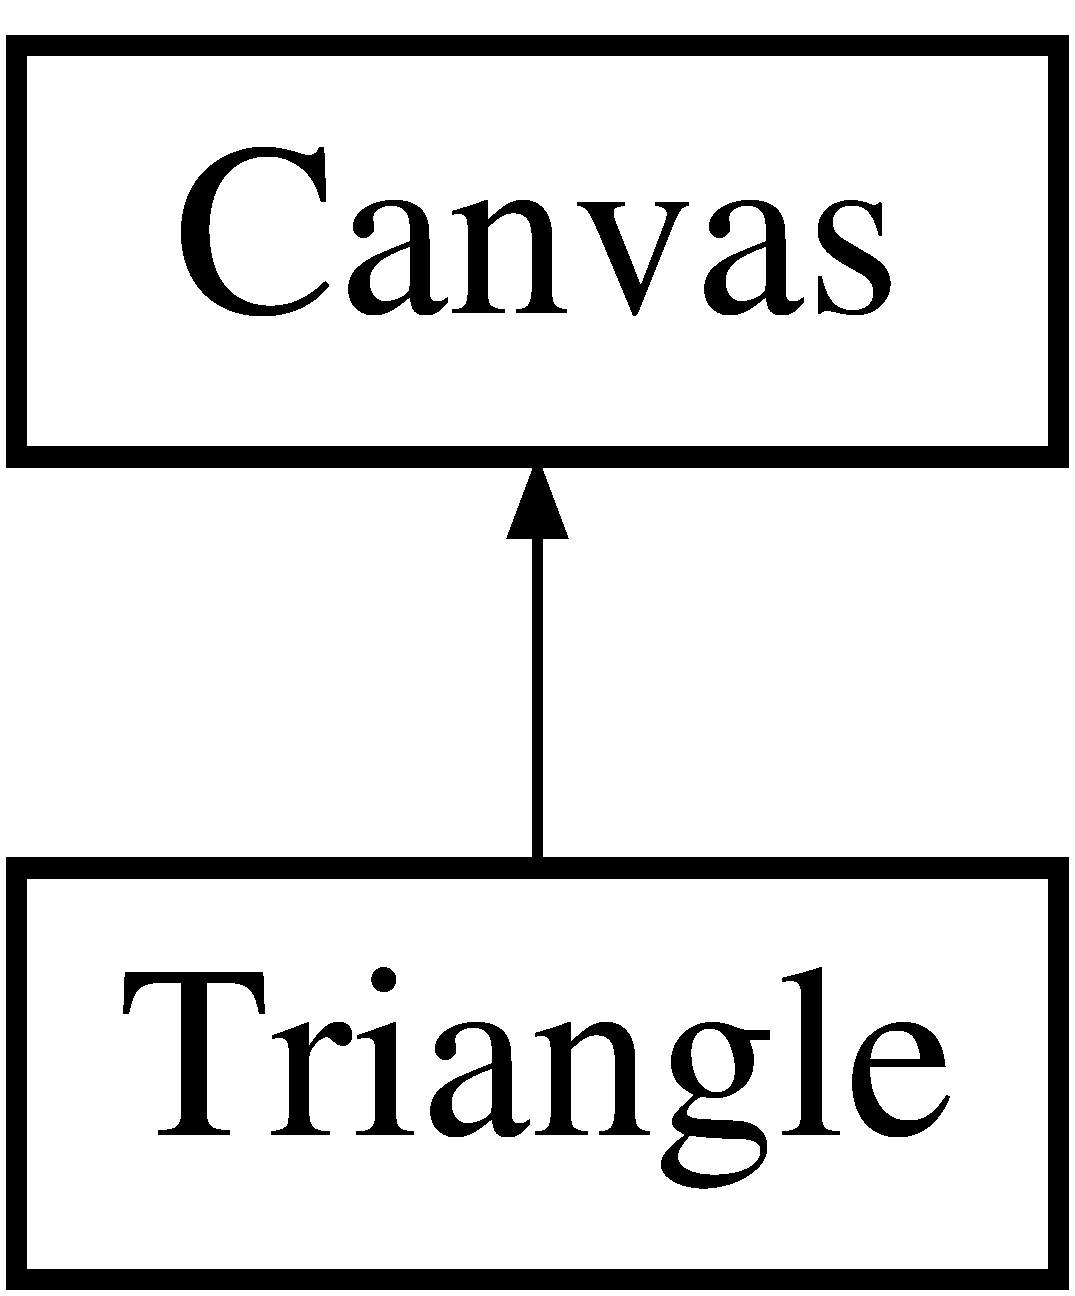
\includegraphics[height=2.000000cm]{class_triangle}
\end{center}
\end{figure}
\subsection*{Public Member Functions}
\begin{DoxyCompactItemize}
\item 
\hypertarget{class_triangle_ac67314c05a3d2d68cf214a72fd8a4655}{{\bfseries Triangle} (\hyperlink{class_target}{Target} $\ast$t, color\-\_\-t bg, \hyperlink{class_best_canvas}{Best\-Canvas} $\ast$bc, \hyperlink{class_config_reader}{Config\-Reader} $\ast$reader)}\label{class_triangle_ac67314c05a3d2d68cf214a72fd8a4655}

\item 
\hypertarget{class_triangle_a31d753323059f2811f7a12aced9edac6}{{\bfseries Triangle} (\hyperlink{class_target}{Target} $\ast$t, color\-\_\-t bg\-\_\-\-Red, color\-\_\-t bg\-\_\-\-Green, color\-\_\-t bg\-\_\-\-Blue, \hyperlink{class_best_canvas}{Best\-Canvas} $\ast$bc, \hyperlink{class_config_reader}{Config\-Reader} $\ast$reader)}\label{class_triangle_a31d753323059f2811f7a12aced9edac6}

\item 
\hypertarget{class_triangle_aba39e11f159609a9dfe8ea9fd6ad5730}{void {\bfseries fast\-Colour\-Technique3} (\hyperlink{struct_r_g_b}{R\-G\-B} target\-Pixel, \hyperlink{struct_r_g_b}{R\-G\-B} canvas\-Pixel, \hyperlink{struct_r_g_b}{R\-G\-B} line\-Color, \hyperlink{struct_coord}{Coord} c)}\label{class_triangle_aba39e11f159609a9dfe8ea9fd6ad5730}

\item 
\hypertarget{class_triangle_a5c5309941f344226f0cb97b5ce66fea9}{void {\bfseries fast\-Colour\-Technique2} (\hyperlink{struct_r_g_b}{R\-G\-B} target\-Pixel, \hyperlink{struct_r_g_b}{R\-G\-B} canvas\-Pixel, \hyperlink{struct_r_g_b}{R\-G\-B} line\-Color, \hyperlink{struct_coord}{Coord} c)}\label{class_triangle_a5c5309941f344226f0cb97b5ce66fea9}

\item 
\hypertarget{class_triangle_af7f44228dc2af65b97affb10c386d85f}{void {\bfseries fast\-Gray\-Technique} (\hyperlink{struct_r_g_b}{R\-G\-B} target\-Pixel, \hyperlink{struct_r_g_b}{R\-G\-B} canvas\-Pixel, \hyperlink{struct_r_g_b}{R\-G\-B} line\-Color, \hyperlink{struct_coord}{Coord} c)}\label{class_triangle_af7f44228dc2af65b97affb10c386d85f}

\item 
\hypertarget{class_triangle_a0f32ca2cdce8d21ada6fd5c5132f9e4a}{void {\bfseries paint\-Canvas} (vector$<$ float $>$)}\label{class_triangle_a0f32ca2cdce8d21ada6fd5c5132f9e4a}

\item 
\hypertarget{class_triangle_a1471eda3739a1f39be9fe59bd93edf96}{void {\bfseries reset\-Canvas} ()}\label{class_triangle_a1471eda3739a1f39be9fe59bd93edf96}

\item 
\hypertarget{class_triangle_af24e0467cbc298ece82c83ab30359d13}{void {\bfseries swip\-Reset\-Convas} (\hyperlink{struct_r_g_b}{R\-G\-B} rgb)}\label{class_triangle_af24e0467cbc298ece82c83ab30359d13}

\item 
\hypertarget{class_triangle_ae3d4e6e9ab7b8145cc605909522f4ecb}{void {\bfseries compute\-Fitness} ()}\label{class_triangle_ae3d4e6e9ab7b8145cc605909522f4ecb}

\item 
\hypertarget{class_triangle_a05b1f62b4b74ff95ccc8d170b5379c9a}{void {\bfseries compute\-Selected\-Fitness} ()}\label{class_triangle_a05b1f62b4b74ff95ccc8d170b5379c9a}

\item 
\hypertarget{class_triangle_a54020e19072de8f07675395b806a82f0}{void {\bfseries compute\-Gray\-Fitness} ()}\label{class_triangle_a54020e19072de8f07675395b806a82f0}

\item 
\hypertarget{class_triangle_a5b4400a2d8f7d2951ac1cc1de41c55bf}{void {\bfseries compute\-Colour\-Fitness} ()}\label{class_triangle_a5b4400a2d8f7d2951ac1cc1de41c55bf}

\item 
\hypertarget{class_triangle_a15d952aa3e44244b734842119fba0fea}{float {\bfseries get\-Fitness} ()}\label{class_triangle_a15d952aa3e44244b734842119fba0fea}

\item 
\hypertarget{class_triangle_a3db7acfcac6a6b7fa92614158c13c0d0}{bool {\bfseries save\-Image} (char $\ast$filename)}\label{class_triangle_a3db7acfcac6a6b7fa92614158c13c0d0}

\item 
\hypertarget{class_triangle_a2dd8a94b9f7803557c395a8f1fd8db77}{bool {\bfseries apply\-Triangle} ()}\label{class_triangle_a2dd8a94b9f7803557c395a8f1fd8db77}

\item 
\hypertarget{class_triangle_aad652cfc36d71b52ce5b7211f9e2364c}{void {\bfseries apply\-Fast\-Shroud} (\hyperlink{struct_coord}{Coord} c, \hyperlink{struct_r_g_b}{R\-G\-B} line\-Color)}\label{class_triangle_aad652cfc36d71b52ce5b7211f9e2364c}

\item 
\hypertarget{class_triangle_afb1ed6bca05869c9c87d8ae28893a35e}{bool {\bfseries barycentric} (\hyperlink{struct_coord}{Coord} c)}\label{class_triangle_afb1ed6bca05869c9c87d8ae28893a35e}

\item 
\hypertarget{class_triangle_a4b3815b250c86f315fe6291e2a232bb6}{void {\bfseries fill\-Up\-Triangle} (float, float, float, float)}\label{class_triangle_a4b3815b250c86f315fe6291e2a232bb6}

\end{DoxyCompactItemize}
\subsection*{Public Attributes}
\begin{DoxyCompactItemize}
\item 
\hypertarget{class_triangle_a4242960824476cbd40ac805a36e72f57}{\hyperlink{struct_r_g_b}{R\-G\-B} {\bfseries line\-Color}}\label{class_triangle_a4242960824476cbd40ac805a36e72f57}

\item 
\hypertarget{class_triangle_ac31e045c63aa605bce528ecd33adb441}{bool {\bfseries flag\-Draw}}\label{class_triangle_ac31e045c63aa605bce528ecd33adb441}

\item 
\hypertarget{class_triangle_a42dd14cfba24d9c5402ee74816d8106d}{int {\bfseries line1}}\label{class_triangle_a42dd14cfba24d9c5402ee74816d8106d}

\item 
\hypertarget{class_triangle_a8dcf84b9e6aac04f46b55f09e385aa2e}{int {\bfseries line2}}\label{class_triangle_a8dcf84b9e6aac04f46b55f09e385aa2e}

\item 
\hypertarget{class_triangle_a30c9ca4ec9dbf12564d1ac061e723dfa}{int {\bfseries line3}}\label{class_triangle_a30c9ca4ec9dbf12564d1ac061e723dfa}

\end{DoxyCompactItemize}
\subsection*{Protected Attributes}
\begin{DoxyCompactItemize}
\item 
\hypertarget{class_triangle_a769752209f8ab14cc98f97b3619dea4c}{\hyperlink{class_config_reader}{Config\-Reader} $\ast$ {\bfseries reader}}\label{class_triangle_a769752209f8ab14cc98f97b3619dea4c}

\end{DoxyCompactItemize}
\subsection*{Additional Inherited Members}


The documentation for this class was generated from the following files\-:\begin{DoxyCompactItemize}
\item 
Triangle.\-h\item 
Triangle.\-cpp\end{DoxyCompactItemize}

%--- End generated contents ---

% Index
\newpage
\phantomsection
\addcontentsline{toc}{part}{Index}
\printindex

\end{document}
